\subsection{Performance Comparison}
%We evaluate QUIC's performance over the standard TCP+TLS stack for adaptive video streaming by playing 175 video clips from YouTube in our testbed. 
For performance comparison between adaptive streaming over \ac{QUIC} and adaptive streaming over \ac{TCP}, we focus on two performance metrics -- (a) video \ac{QoE}, and (b) data download and data wasted due to quality switching. 
%In this section, at first, we evaluate Google's claims about the QUIC by comparing it with normal TCP connection.  After that, we compare data wastage while playing video for the normal TCP based connection and the QUIC based connection.

\subsubsection{Does QUIC Improve Video QoE?}
%Here we compare four different QoE metric of video streaming network standard TCP+TLS stack and QUIC stack. These metrics are i) number of quality switches, ii) overall playback quality (bitrate), iii) rebuffering count and iv) data wastages.
%After playing all the videos in both TCP+TLS stack and QUIC stack, we have first analyzed the following three different performance metrics to check how the streaming performance differs for the two protocol stacks.   
We quantify video quality using three parameters which impact \ac{QoE}~\cite{balachandran2012quest}.
\begin{enumerate}[leftmargin=*]
	\item\textbf{Video Quality Switches:} For adaptive video streaming, the streaming client dynamically adapts the video quality based on the environment (like available channel bandwidth). If the number of quality switching is high, then it negatively impacts the video QoE. 
	\item\textbf{Playback Quality:} We measure what proportion of the video that is played at the highest possible bitrate. 
	\item\textbf{Rebuffering Events:} We measure the number of times the playback buffer is completely used up and triggers rebuffering.
\end{enumerate}
%As mentioned in~\cite{balachandran2012quest}, these three metrics give a good indication of QoE for video streaming applications. 

\subsubsection{Video Quality Switch}
\begin{figure}[!t]
    \captionsetup[subfigure]{}
    \begin{center}
%        \subfloat[\label{fig:reschange_up}Quality Improvements]{
%            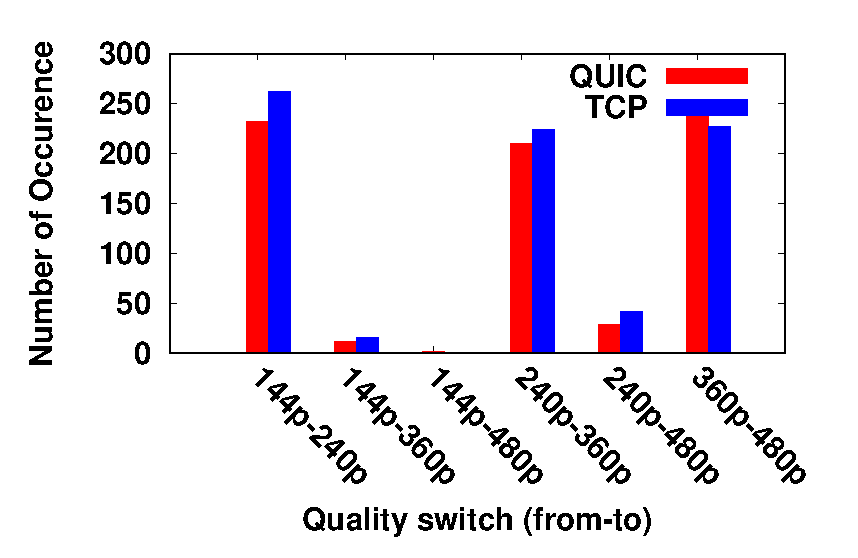
\includegraphics[width=0.48\linewidth]{img/metric/reschange_up}
%        }
%        \subfloat[\label{fig:reschange_down}Quality Drops]{
%            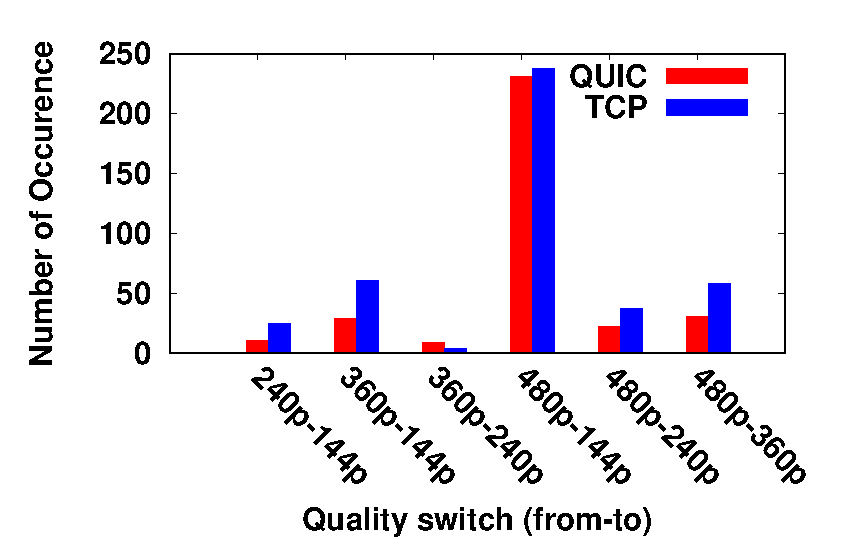
\includegraphics[width=0.48\linewidth]{img/metric/reschange_down}
%        }
        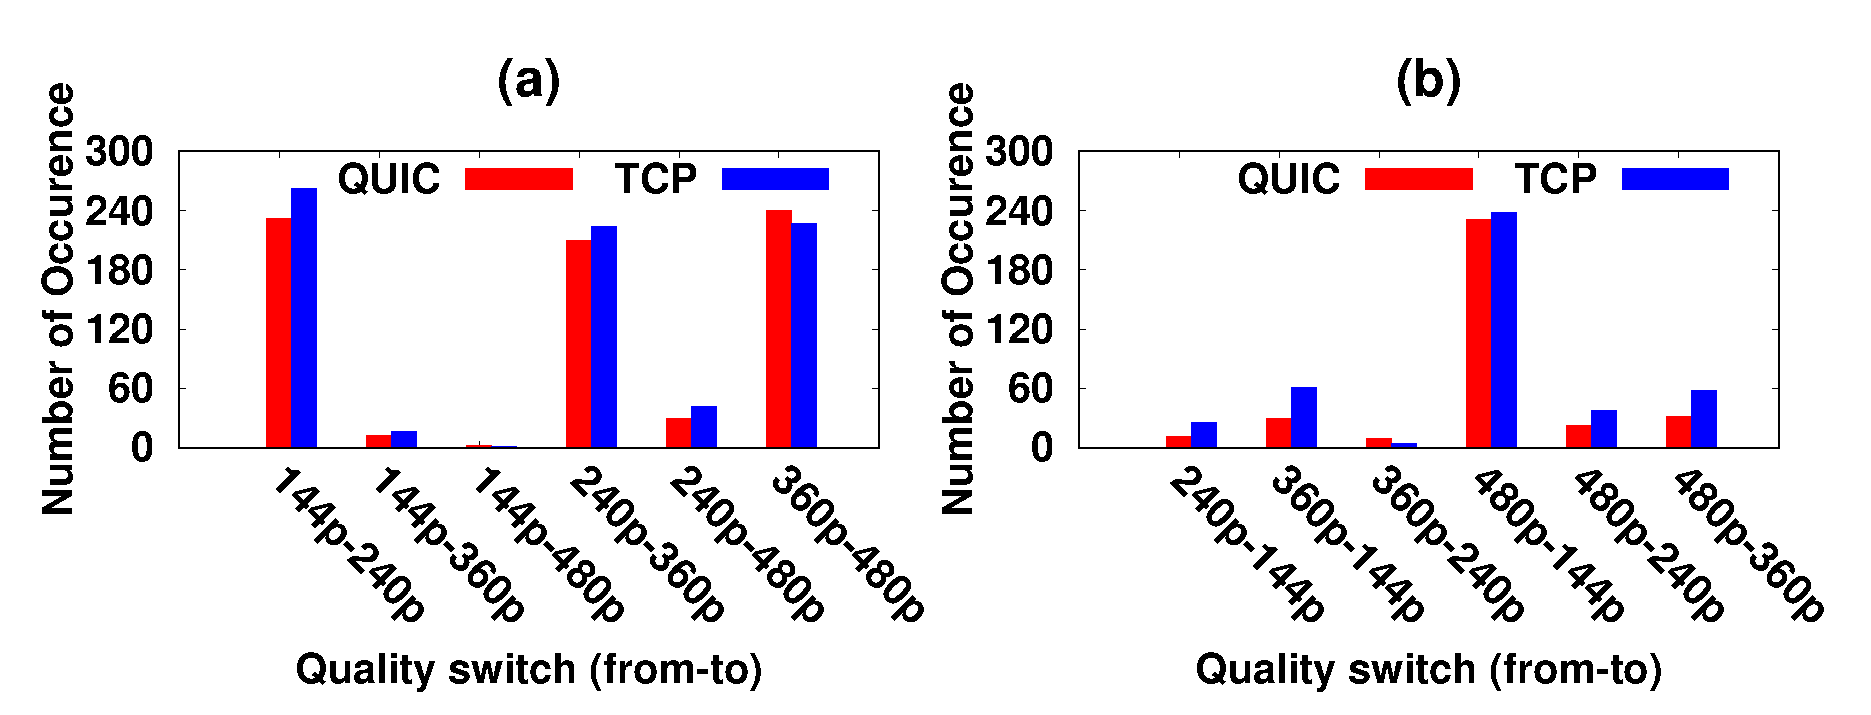
\includegraphics[width=0.9\linewidth]{img/plotdata/metric/reschange_up_down}
        \caption{\label{fig:reschange}Quality switching: (a) Quality upgrade, (b) Quality drop}
    \end{center}
\end{figure}

%\begin{figure}[!t]
%    \captionsetup[subfigure]{}
%    \begin{center}
%%        \subfloat[\label{fig:reschange_up_percent}Quality Improvements]{
%%            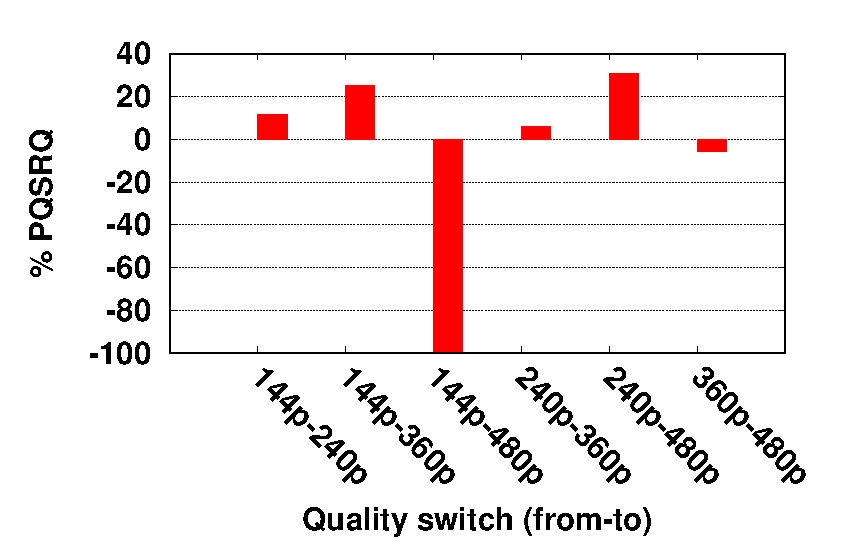
\includegraphics[width=0.48\linewidth]{img/metric/reschange_up_percent}
%%        }
%%        \subfloat[\label{fig:reschange_down_percent}Quality Drops]{
%%            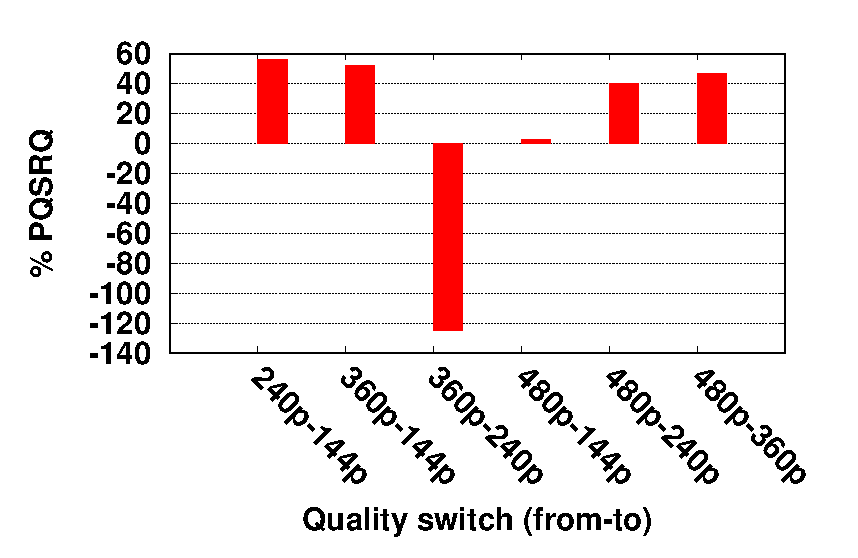
\includegraphics[width=0.48\linewidth]{img/metric/reschange_down_percent}
%%        }
%        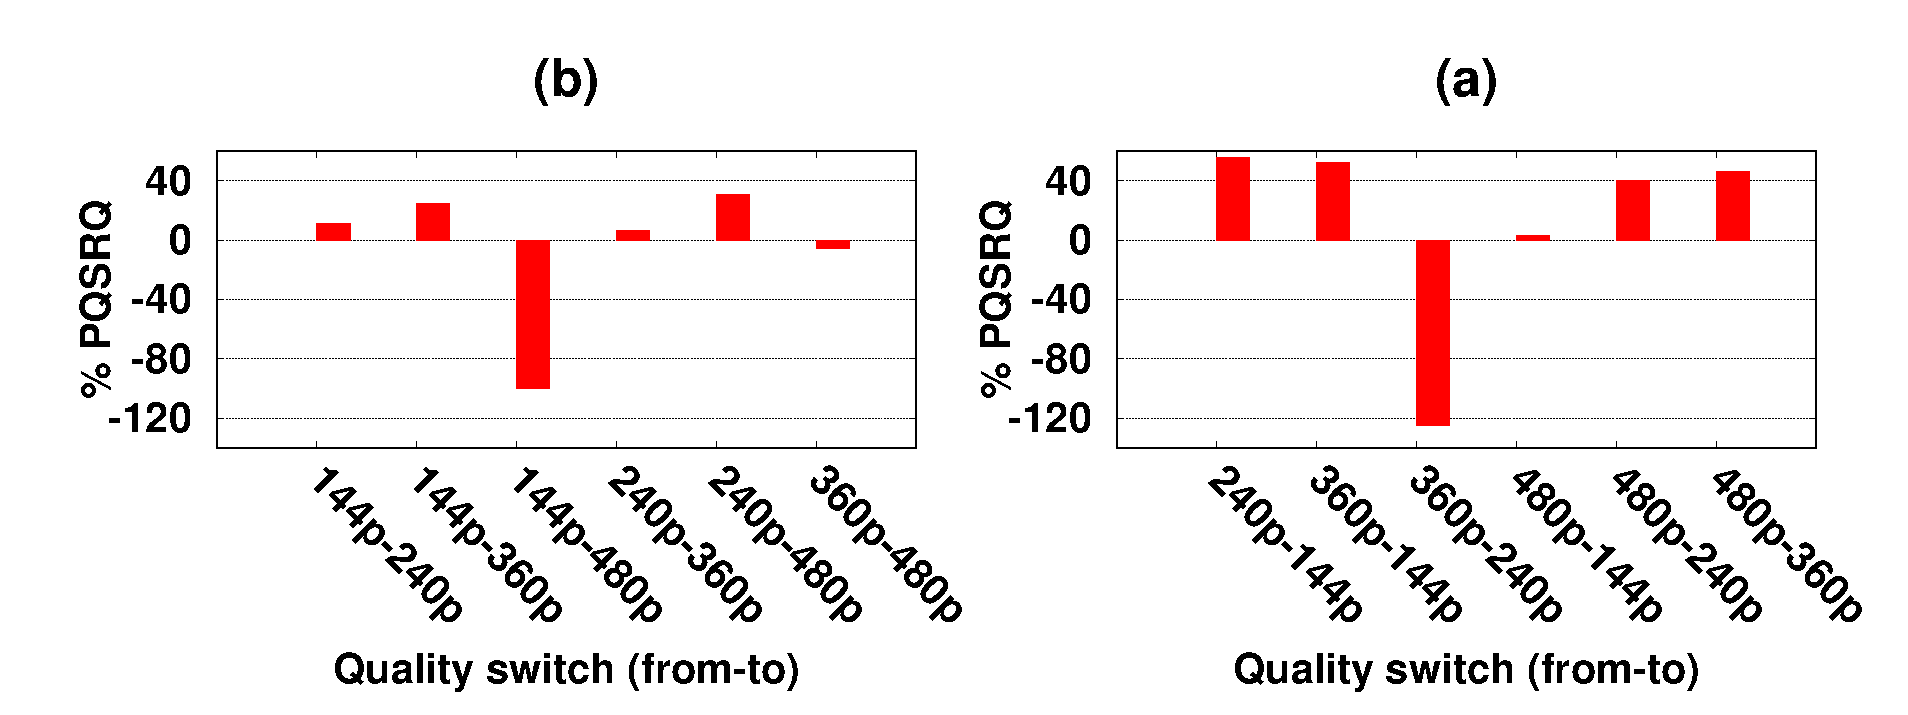
\includegraphics[width=\linewidth]{img/plotdata/metric/reschange_up_down_percent}
%        \caption{\label{fig:reschange_percent}Percentage quality switch reduction with QUIC: (a) Quality upgrade, (b) Quality drop}
%    \end{center}
%\end{figure}

We compare the number of switches in video quality, both in terms of quality upgrades and quality drops, as shown in \fig\ref{fig:reschange}.
We observe that \ac{QUIC} incurs less quality switches than that of \ac{TCP} for almost all the cases. 
%To quantify the improvement in quality switching with QUIC, we define a metric called \textit{Percentage Quality Switch Reduction with QUIC} (PQSRQ) which is defined as follows. For two quality levels $\mathcal{Q}_1$ and $\mathcal{Q}_2$, let $QSQ(\mathcal{Q}_1,\mathcal{Q}_2)$ and and $QST(\mathcal{Q}_1,\mathcal{Q}_2)$ denote the number of quality switch from $\mathcal{Q}_1$ to $\mathcal{Q}_2$ with QUIC and TCP, respectively.  Then, $PQSRQ(\mathcal{Q}_1,\mathcal{Q}_2) = \frac{QSQ(\mathcal{Q}_1,\mathcal{Q}_2)}{QST(\mathcal{Q}_1,\mathcal{Q}_2)} \times 100\%$. \fig\ref{fig:reschange_percent} plots the value of PQSRQ for various quality levels, both during quality improvements and quality drops. We observe that 
It is evident from the figure that for some quality levels, the percentage reduction in quality switches is more than $20\%$ during quality upgrades, and more than $40\%$ during quality drops. For the few cases when \ac{QUIC} performs worse than \ac{TCP}, we actually note that the number of data points for those quality levels is less in our collected dataset. Interestingly, in terms of percentage quality switch reduction, \ac{QUIC} outperforms \ac{TCP}  more during quality drops compared to quality upgrades, which is an indication of good \ac{QoE}.  Nevertheless, it is expected that the overall playback quality should be biased towards the high quality video segments for supporting better viewing experiences to the end users, which we explore next. 

\subsubsection{Video Quality During Playback}
%\begin{figure}[!t]
%    \centering
%    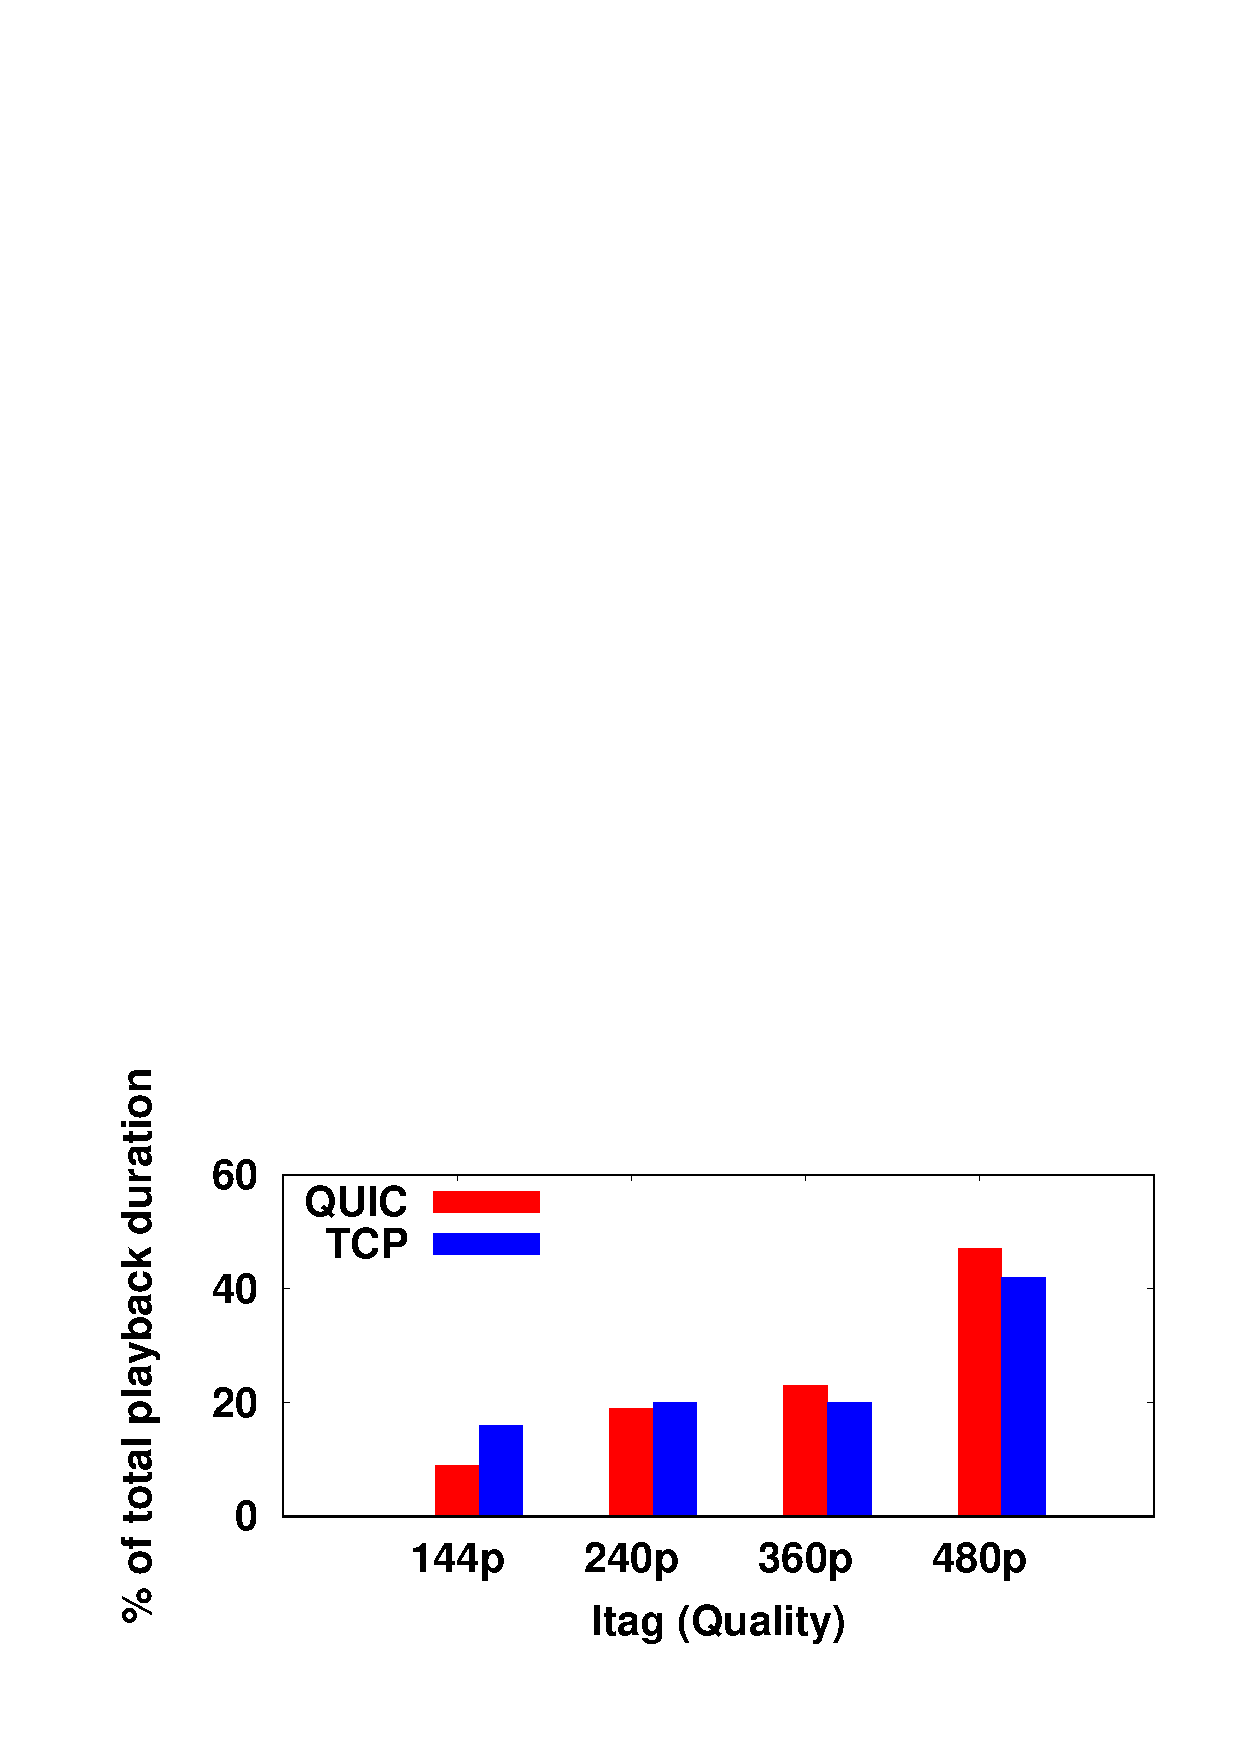
\includegraphics[width=\linewidth]{img/metric/time_duration_percent}
%    \caption{Overall playback Time of Each Quality \notesc{convert this to percentage - (data downloaded for a particular quality / total data downloaded for all the qualities) x 100\%} \noteam{Done.}}
%    \label{fig:avg_bitrate}
%\end{figure}

\begin{figure}[!t]
	\captionsetup[subfigure]{}
	\begin{center}
%		\subfloat[\label{fig:avg_bitrate}\% Playback Time]{
%			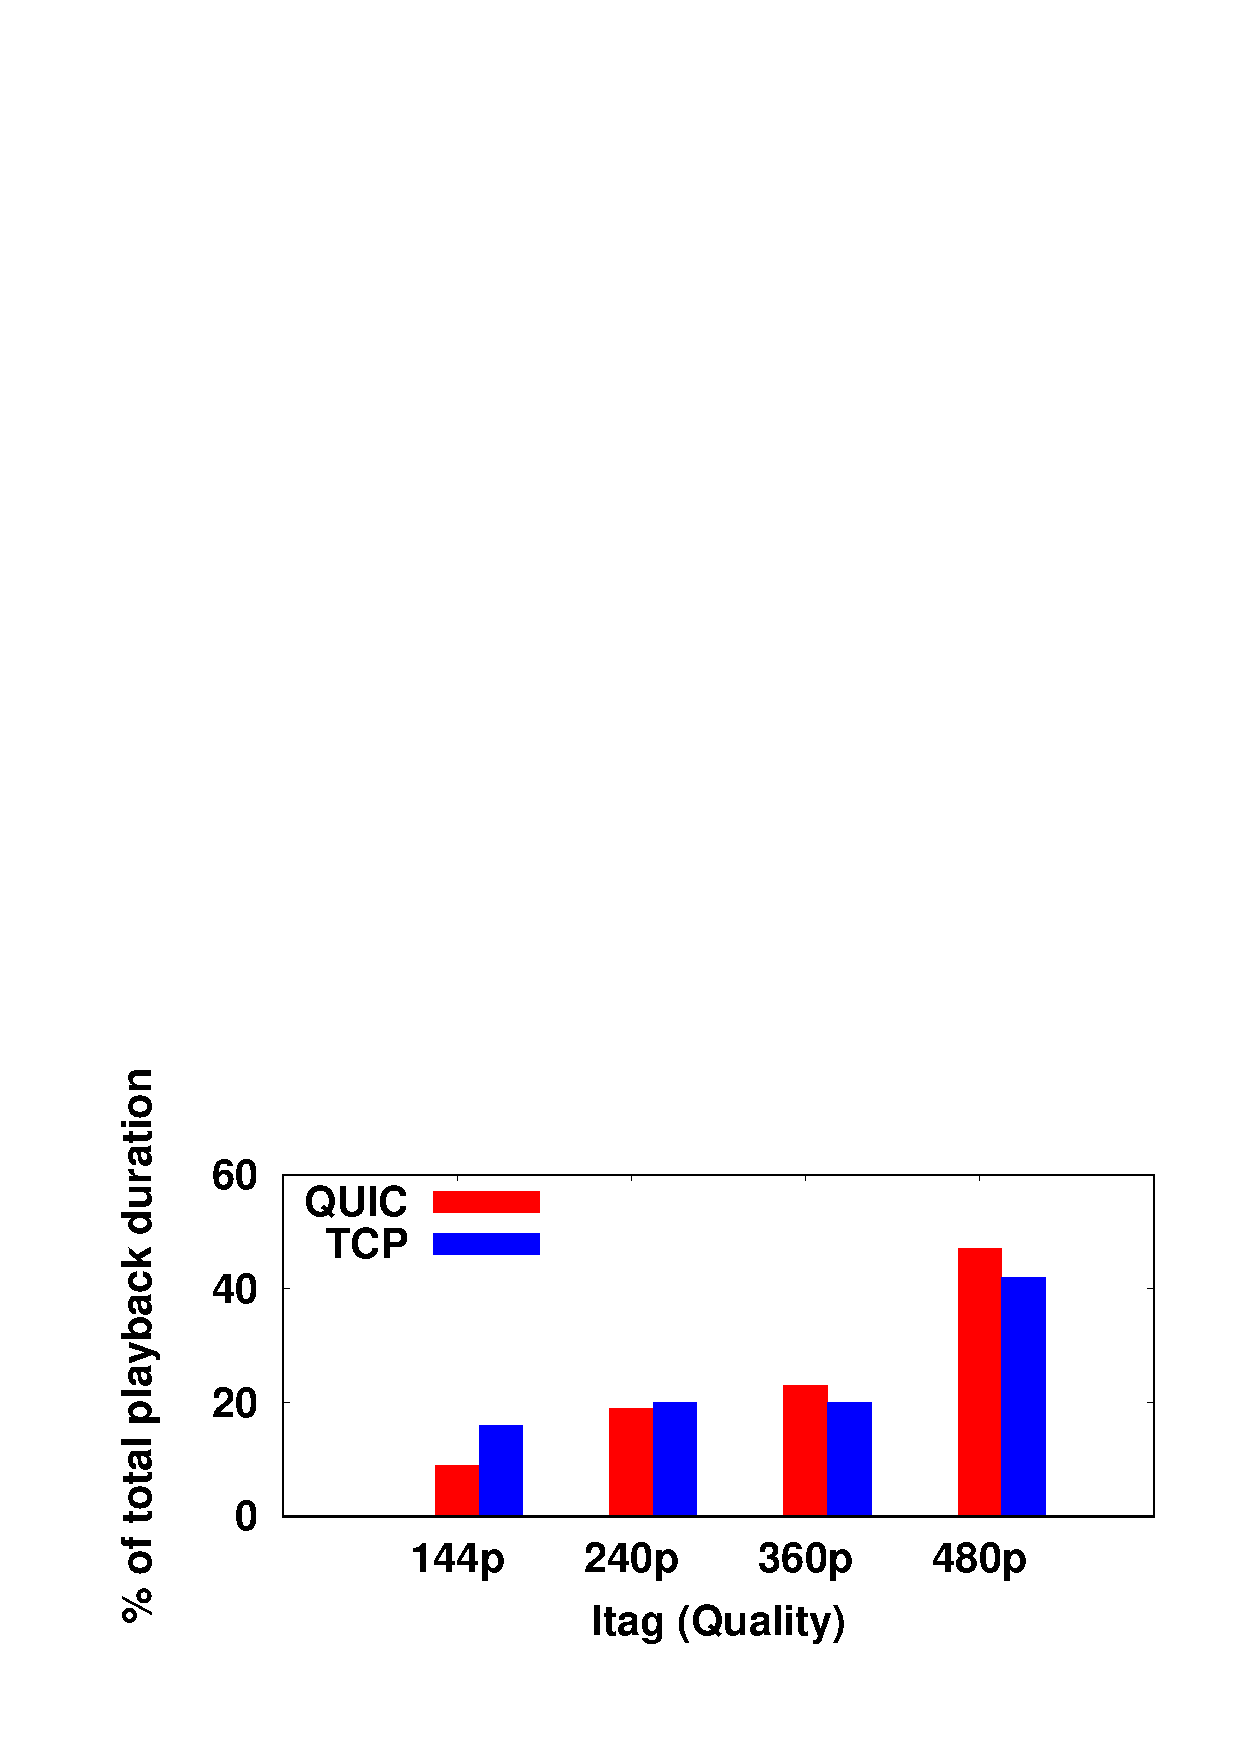
\includegraphics[width=0.48\linewidth]{img/metric/time_duration_percent}
%		}
%		\subfloat[\label{fig:rebuffering}Rebuffering Count]{
%			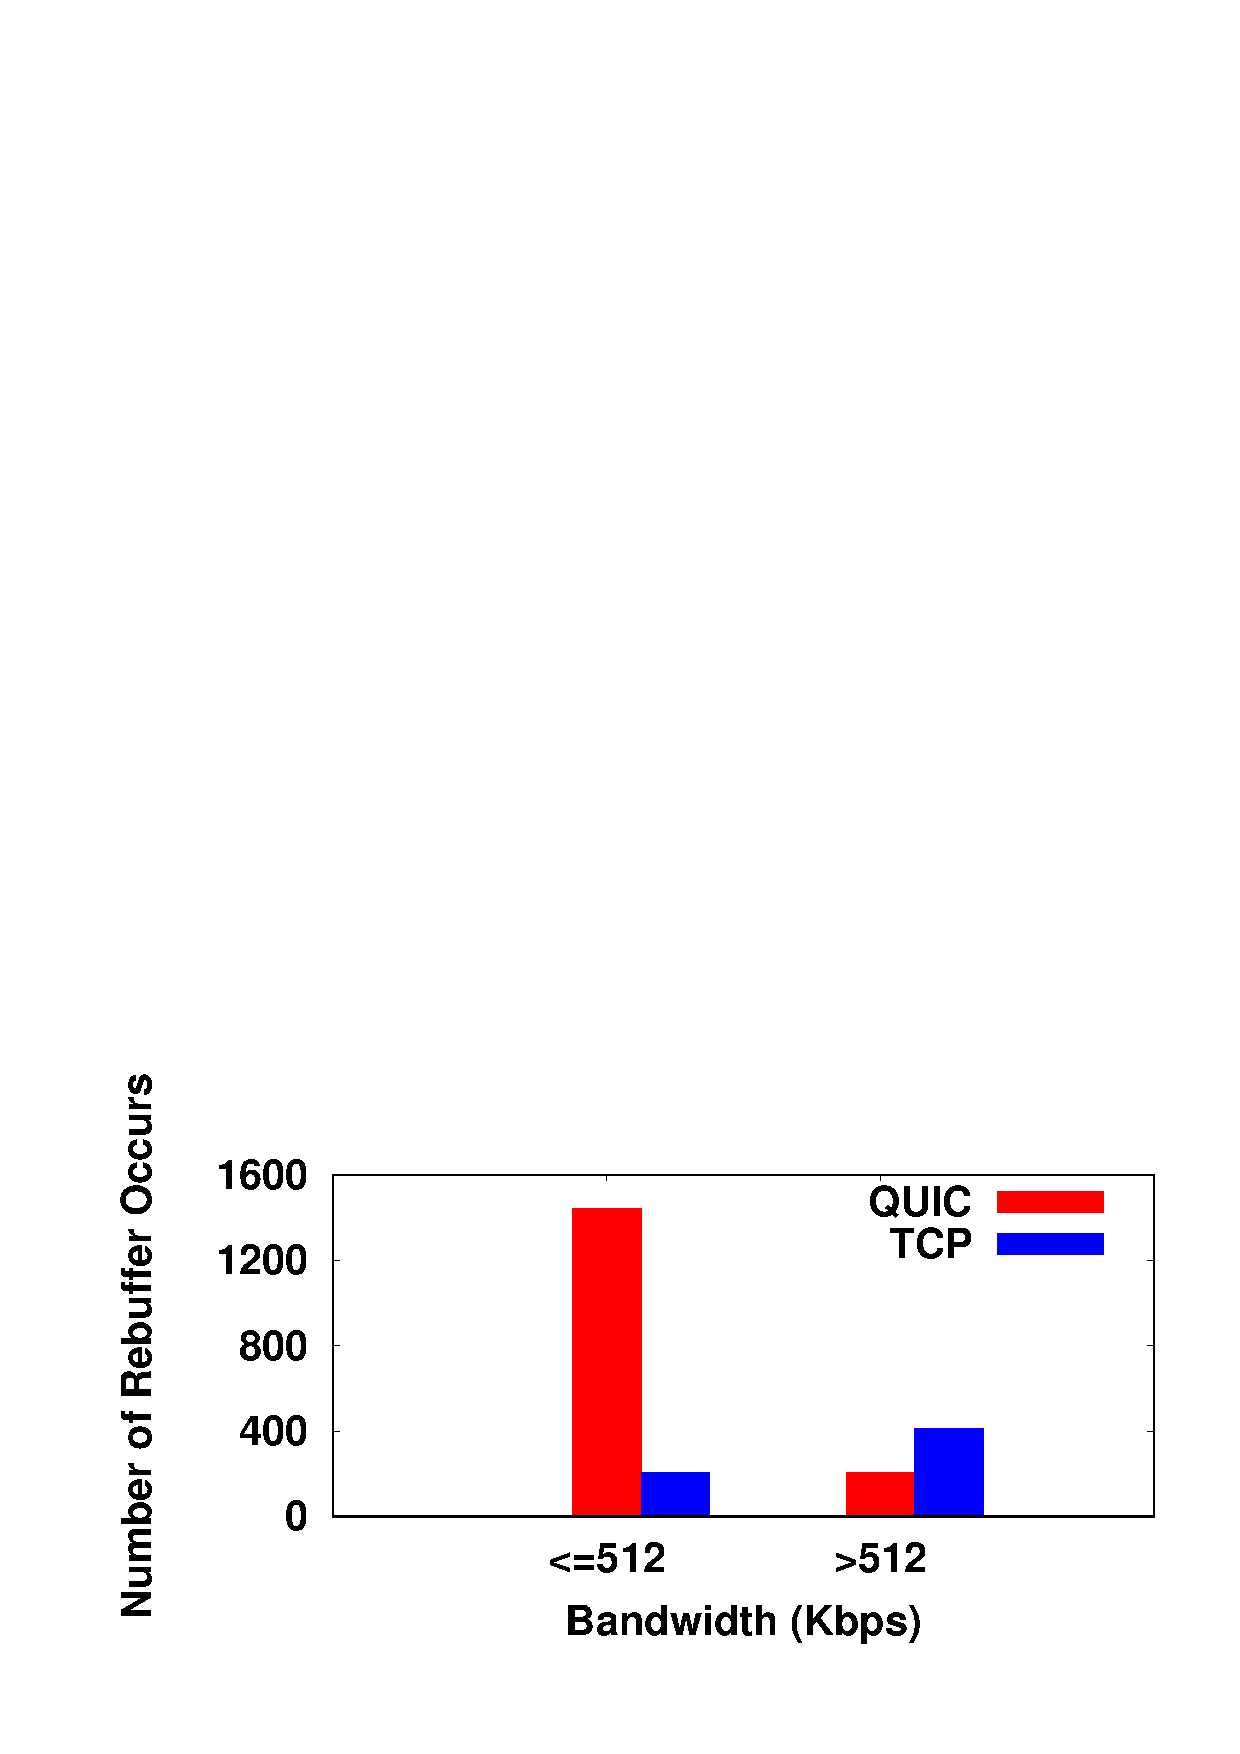
\includegraphics[width=0.48\linewidth]{img/metric/rebuffering}
%		}
        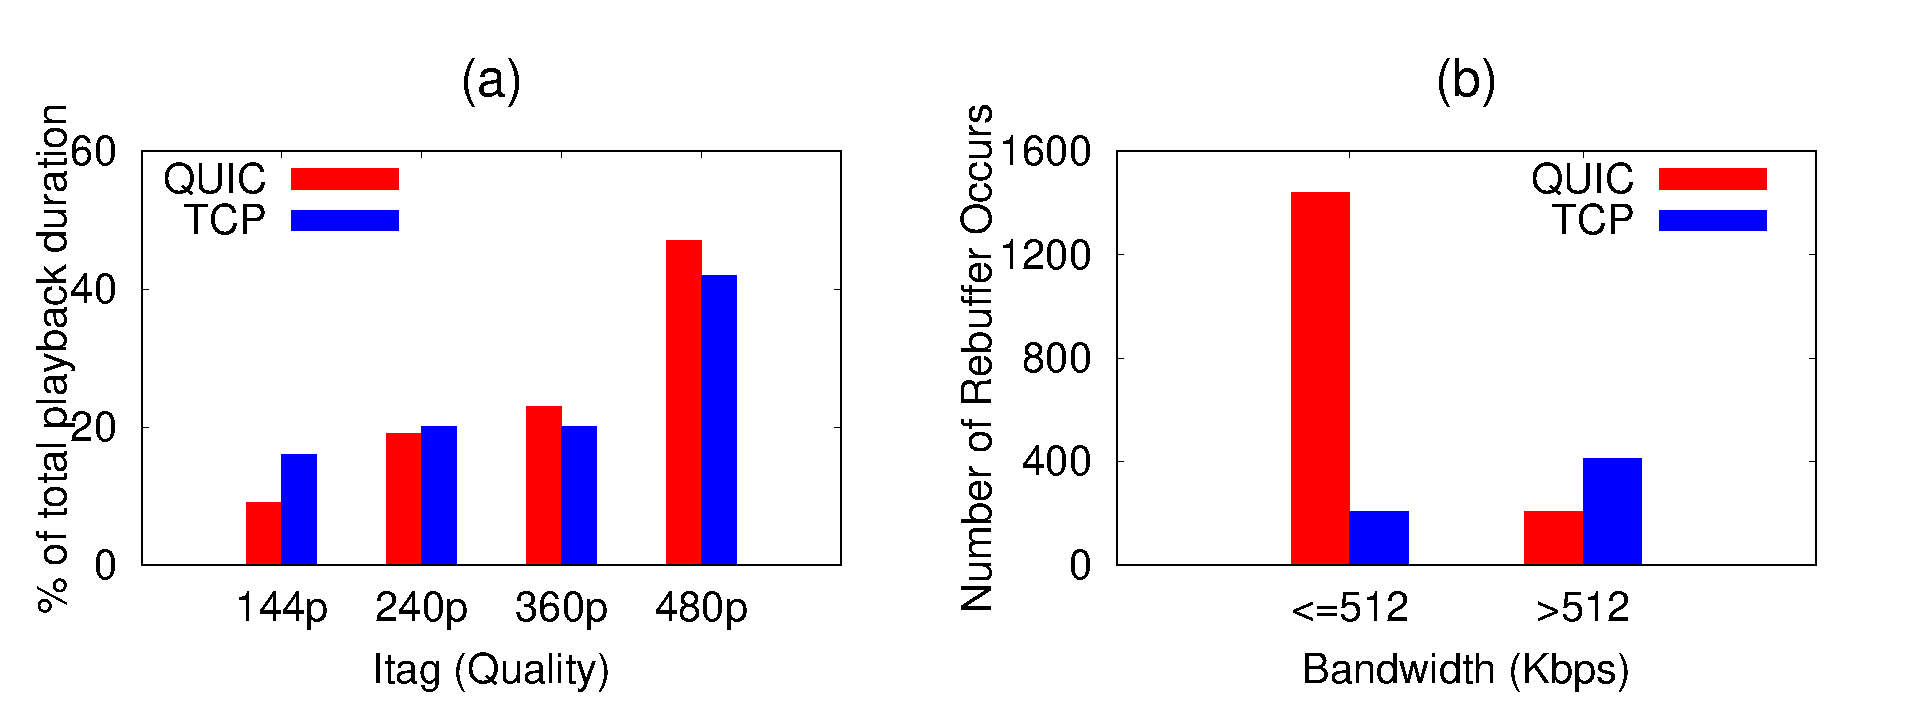
\includegraphics[width=0.9\linewidth]{img/plotdata/metric/time_duration_percent_rebuffering}
		\caption{\label{fig:bitrate_rebuffering}(a) Overall playback time,  (b) Rebuffering}
	\end{center}
\end{figure}

We investigate how long does a video play at a different video quality levels.
\fig\ref{fig:bitrate_rebuffering}(a) shows the percentage of total playback time at each video quality. 
Note that under similar experiment conditions, \ac{QUIC} enabled player plays the video at higher resolution compared to \ac{TCP}. Therefore, it provides better \ac{QoE} compared to \ac{TCP} for adaptive streaming in terms of quality switching and overall playback quality. 

%We compare the total playback time for streaming over QUIC and streaming over TCP, and we observe that QUIC is biased towards the high quality video segments. It can be noted here that during the data collection phase, we have ensured that a video should experience similar bandwidth throttling with respect to time ($\pm 10 Kbps$ deviation with respect to time, as mentioned earlier), when downloaded through both QUIC and TCP. Therefore, \fig\ref{fig:avg_bitrate} and \fig\ref{fig:reschange} together ensure that while QUIC reduces switching between video qualities, it tends to download video segments with higher quality values under the similar network bandwidth availability. Therefore, it provides better QoE compared to TCP for adaptive streaming in terms of quality switching and overall playback quality. 


\subsubsection{Rebuffering}
%\begin{figure}[h!]
%\centering
%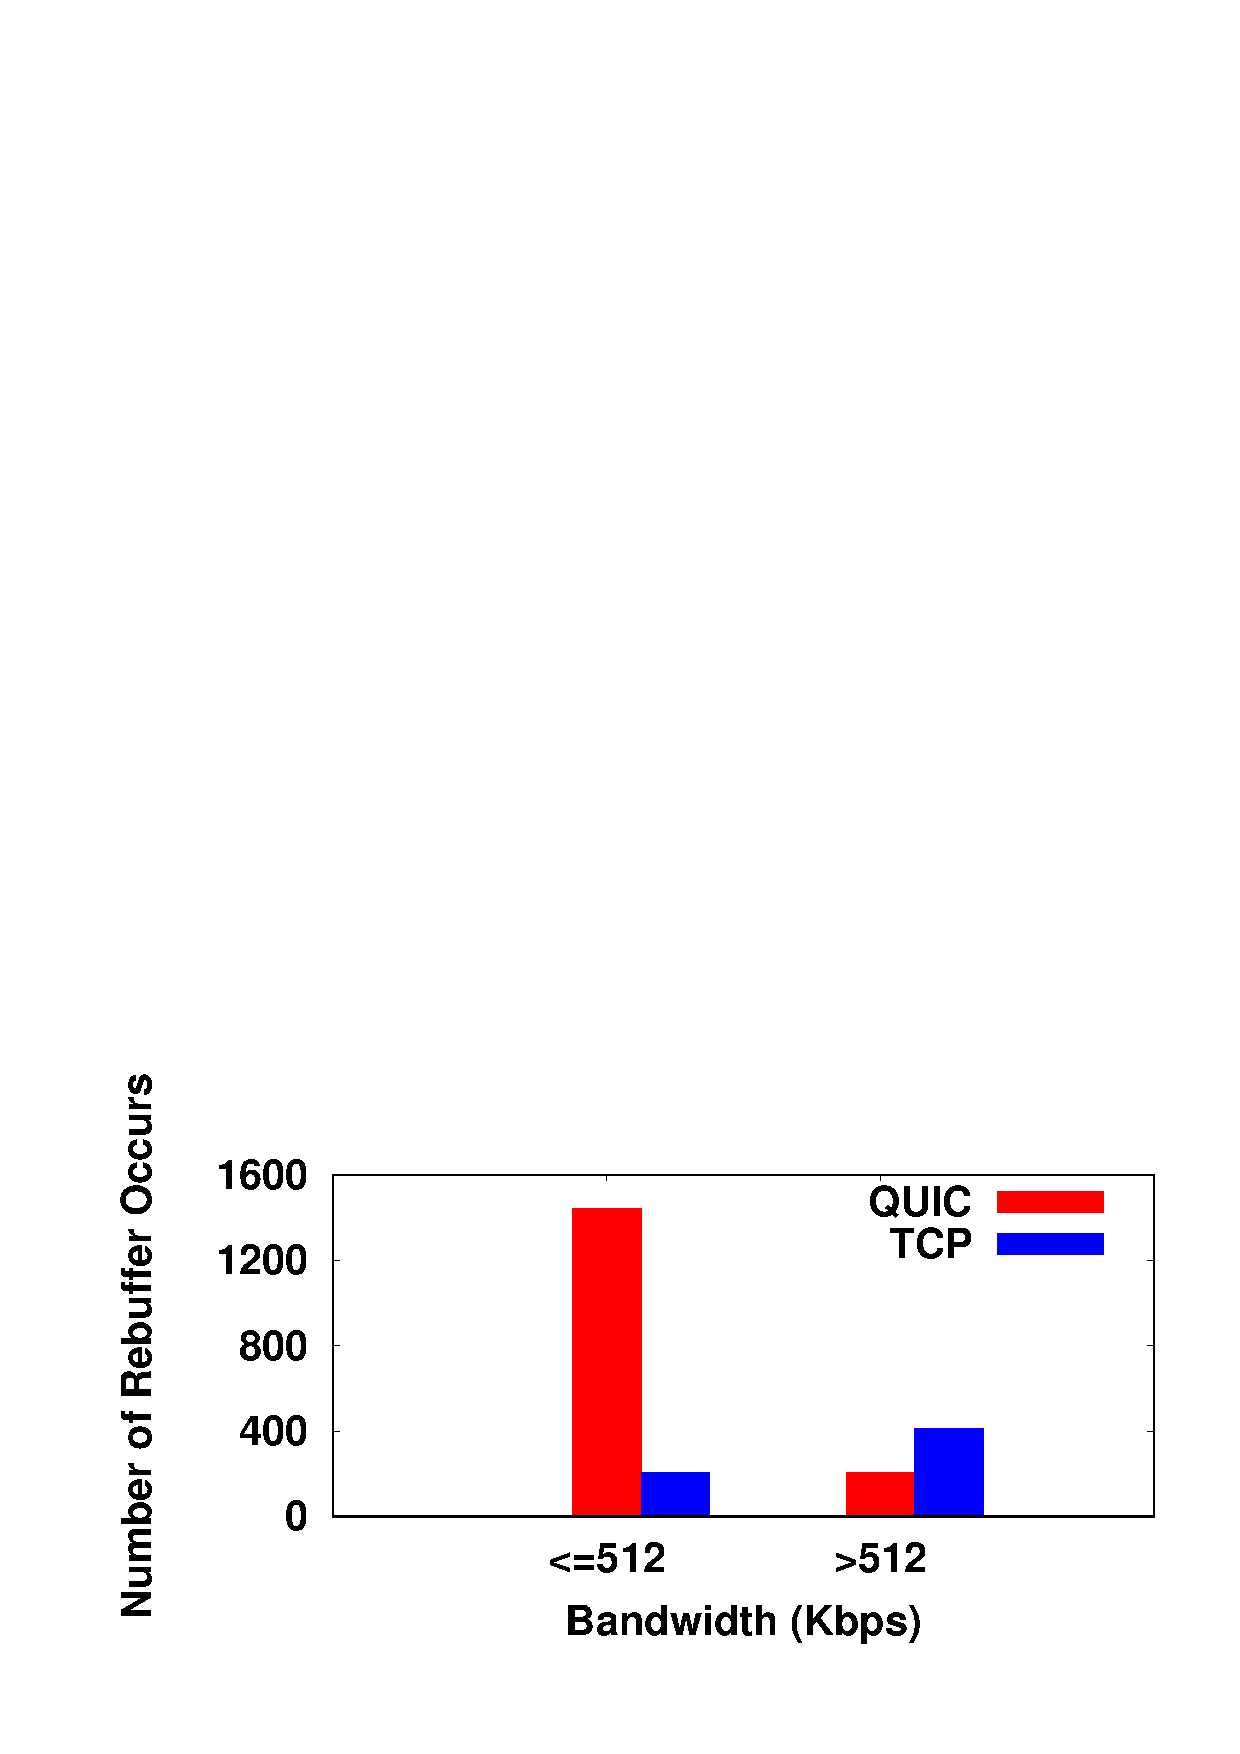
\includegraphics[width=\linewidth]{img/metric/rebuffering}
%\caption{Rebuffering Count in Different Bandwidth Levels \notesc{Show two scenarios -- (a) bandwidth less than 512 Kbps and (b) bandwidth greater than 512 Kbps}\noteam{Done.}}
%\label{fig:rebuffering}
%\end{figure}

%\begin{table}[h!]
%    \centering
%    \caption{Rebuffering}
%    \label{table:rebuffering}
%    \begin{tabular}{||c|c|c|}
%        \hline
%        Bandwidth & QUIC & TCP \\\hline\hline
%        64 & 1236 & 205 \\\hline
%        404 & 206 & 0 \\\hline
%        744 & 0 & 0 \\\hline
%        1084 & 0 & 0 \\\hline
%        1424 & 206 & 410 \\\hline
%        Total & 1648 & 615 \\\hline
%    \end{tabular}
%\end{table} 

We counted the number of rebuffering events during playback for both \ac{QUIC} and \ac{TCP} enabled streaming.
We used two bandwidth settings: (a) low bandwidth at less than 512 Kbps, (b) high bandwidth at greater than 512 Kbps.
\fig\ref{fig:bitrate_rebuffering}(b) shows the frequency of rebuffering events.
When the channel bandwidth is less than $512$ Kbps, QUIC shows runs out of buffered data more frequently than TCP. 
Since QUIC tries to maintain a high video quality, therefore, even at low bandwidth it does not quickly switch to a low bitrate leading to buffer depletion and triggers rebuffering.

%Next we observe another important and critical QoE metric, which is rebuffering count. During a rebuffering event, the streaming client's playback buffer becomes zero, and the video rendering halts at this point, resulting in poor QoE. As rebuffering depends on the available channel bandwidth along with current playback quality, we plot total rebuffering counts over all the dataset for two different bandwidth levels -- (a) channel bandwidth less than  $512$ Kbps and (b) channel bandwidth greater than $512$ Kbps. The resultant plot is shown in \fig\ref{fig:rebuffering}. We have interesting observation here. When the channel bandwidth is less than $512$ Kbps, QUIC shows significantly higher numbers of rebuffering events compared to TCP. On contrary, with channel bandwidth more than $512$ Kbps, QUIC performs better than TCP. So, in terms of rebuffering, we can say that QUIC performs poorly compared to TCP when channel quality is bad. Incidentally, we observe that QUIC tries to download high quality videos even at low bandwidth availability, which we presume as one of the reasons for the large number of rebuffering events.  

In summary, we observe that although \ac{QUIC} tries to download high quality videos even at low bandwidth availability and reduces number of quality switches during adaptive streaming, it can significantly increase the rebuffering events when video quality if low. 
If this rebuffering count goes beyond a threshold, \ac{QoE} for the video streaming application may suffer. 
As the rebuffering count during the video streaming over \ac{QUIC} is significantly higher than that of \ac{TCP}, when channel quality is poor, we conclude that \ac{QUIC} may not improve overall video \ac{QoE} under all conditions. 

%
%Rebuffering is the most critical QoE metric for video streaming. Before the age of dynamic adaptation begins, rebuffering was the only QoE metric. So, we also compared rebuffering count in the \fig\ref{fig:rebuffering} and the \tbl\ref{table:rebuffering}. We found that QUIC rebuffers more for lower bandwidth. It happens because QUIC tries to higher quality for longer playback time. However, TCP is more conservative than QUIC. So, QUIC does not perform well enough here.

\subsection{Impact of ABR Streaming over Data Consumption: QUIC vs TCP}

%Adaptive video streaming improves QoE by dynamically adapting video quality levels based on available channel bandwidth, however it has a direct implication of the amount of data that is downloaded at the client side. 
Existing studies on adaptive video streaming has shown that the complete data, which is downloaded by the streaming media client, is not utilized during the actual video playback~\cite{krishnappa2013dashing}. 
%A significant amount of data is wasted during the quality adaptation, as the streaming clients use a conservative approach during quality switching. 
In this section, we discuss the performance of adaptive streaming over \ac{QUIC} and \ac{TCP} in terms of data consumption. 

\begin{figure}[!t]
	\captionsetup[subfigure]{}
	\begin{center}
%		\subfloat[\label{fig:down_quality} At Different Quality]{
%			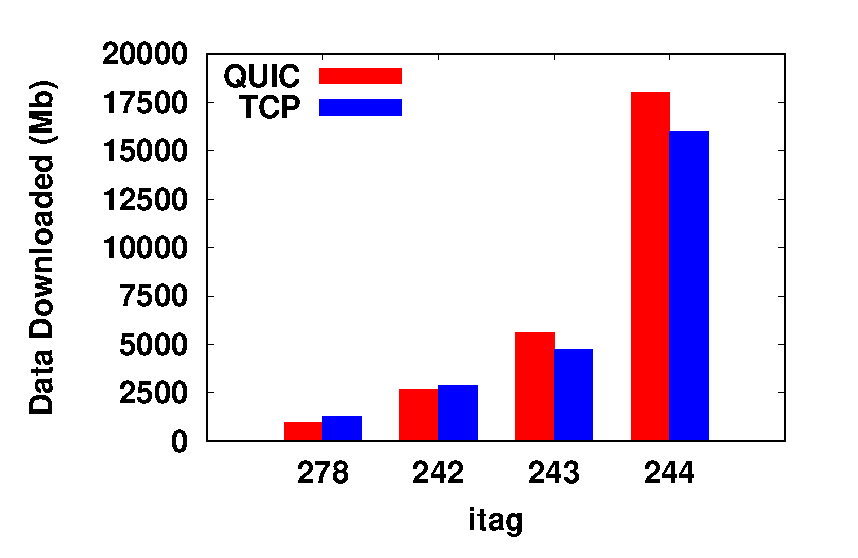
\includegraphics[width=0.48\linewidth]{img/CDF/Data_Dowloaded}
%		}
%		\subfloat[\label{fig:down_band}At Different Bandwidth]{
%			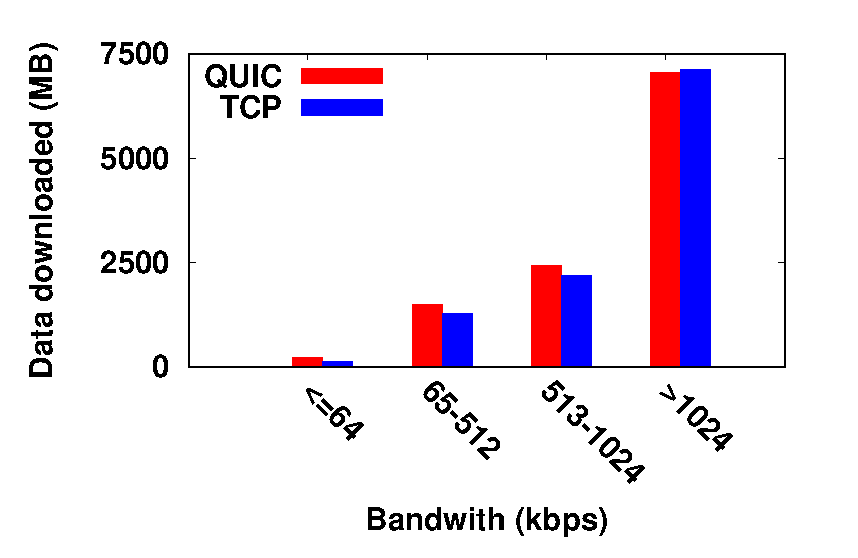
\includegraphics[width=0.48\linewidth]{img/CDF/data_downloaded_bw}
%		}
        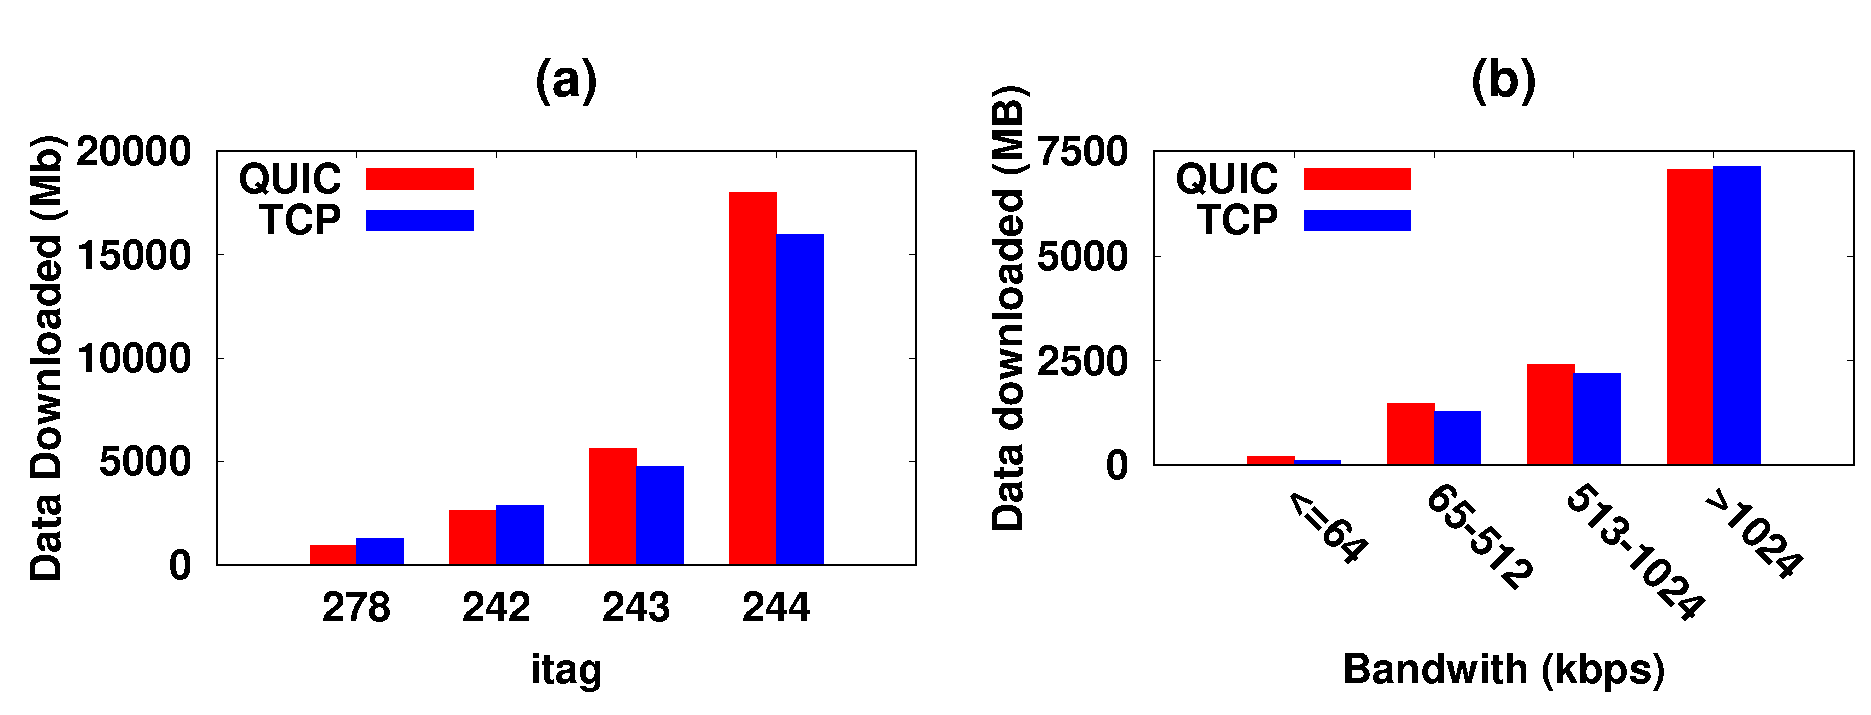
\includegraphics[width=0.9\linewidth]{img/plotdata/CDF/downloaded/data_dowloaded_itag_bw}
		\caption{\label{fig:data_download}Data downloaded: (a) Different quality levels, (b) Different channel bandwidth}
	\end{center}
\end{figure}


\subsubsection{Data Download for Adaptive Video Streaming}
We first look into the total data downloaded with \ac{QUIC} and \ac{TCP} during the playback of same set of videos under similar channel conditions. \fig\ref{fig:data_download}(a) shows the total data downloaded for different quality levels, and \fig\ref{fig:data_download}(b) plots the total data downloaded under various channel conditions in terms of bandwidth availability. We observe that \ac{QUIC} downloads more data under itag value $243$ and $244$ which are the best quality levels observed in the collected data set. 
%We then look into the total data download under various network conditions (channel bandwidth availability). \fig\ref{fig:down_band} plots the total amount of data downloaded over all the sampled videos grouped into four different available bandwidth conditions. 
Further, the figure indicates that the total data downloaded with \ac{QUIC} is high compared to \ac{TCP} when the available channel bandwidth is less than $1$ Mbps. Therefore, we hypothesize that with \ac{QUIC} enabled YouTube streaming can download high quality videos even at the low network quality. 
However, as we mentioned earlier, there is a possibility of data wastage during the quality switching with adaptive video streaming over the web. Next, we first explain the reason for this data wastage, and then we go for a thorough analysis of the data wastage for the two protocols. 

%Let us look at the total data downloaded (\fig\ref{fig:rabuf761856q}) by QUIC and TCP and the data wasted (\fig\ref{fig:rabuf76q1}) by both the protocols. Data wasted is computed by considering the fact that if there is lower resolution data when a higher resolution is being played then the lower resolution data is being wasted. The amount of data downloaded and data wasted has been calculated using the bit rates available for each itag in the HAR files.

%\begin{figure}[ht!]
%	\centering
%	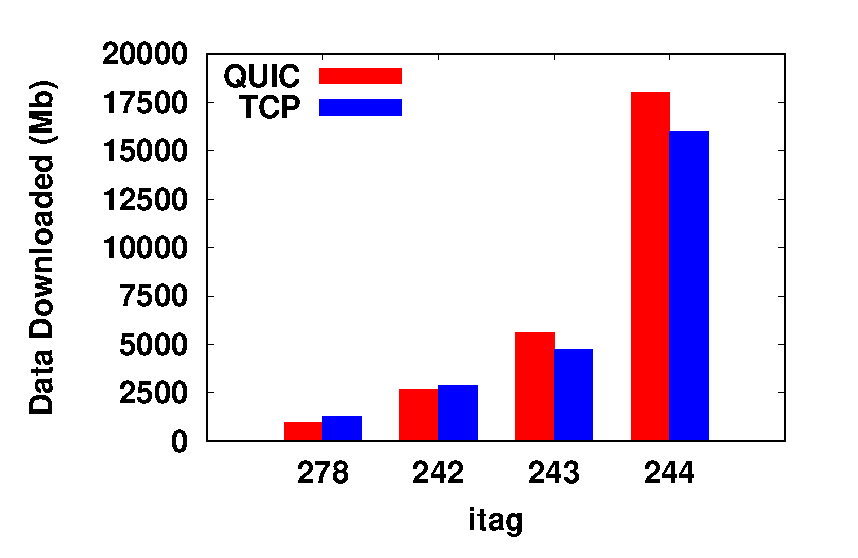
\includegraphics[width=0.9\linewidth]{img/CDF/Data_Dowloaded}
%	\caption{Amount of Data Downloaded}
%	\label{fig:rabuf761856q}
%\end{figure}


%\notesc{Total data downloaded at various bandwidth buckets --  (a) $\leq 64$ Kbps, (b) $65-512$ Kbps, (c) $513-1024$ Kbps, (d) $> 1024$ Kbps}

\subsubsection{Why There is a Possibility of Data Waste During Adaptive Streaming?}


%\begin{figure}[!t]
%	\captionsetup[subfigure]{}
%	\begin{center}
%		\subfloat[\label{fig:rseg1Q}QUIC]{
%			\includegraphics[width=0.48\linewidth]{img/QUICPlots/plot_timerange}
%		}
%		\subfloat[\label{fig:rsegr1T}TCP]{
%			\includegraphics[width=0.48\linewidth]{img/TCPPlots/plot_timerange}
%		}
%		
%		\caption{\label{fig:rserr1}Plot for \textit{Time Range} over time for a YouTube video of id $<$OJZgOOOE1zY$>$ \notesc{The fonts need to be clear}}
%	\end{center}
%\end{figure}
\begin{figure}[!t]
\centering
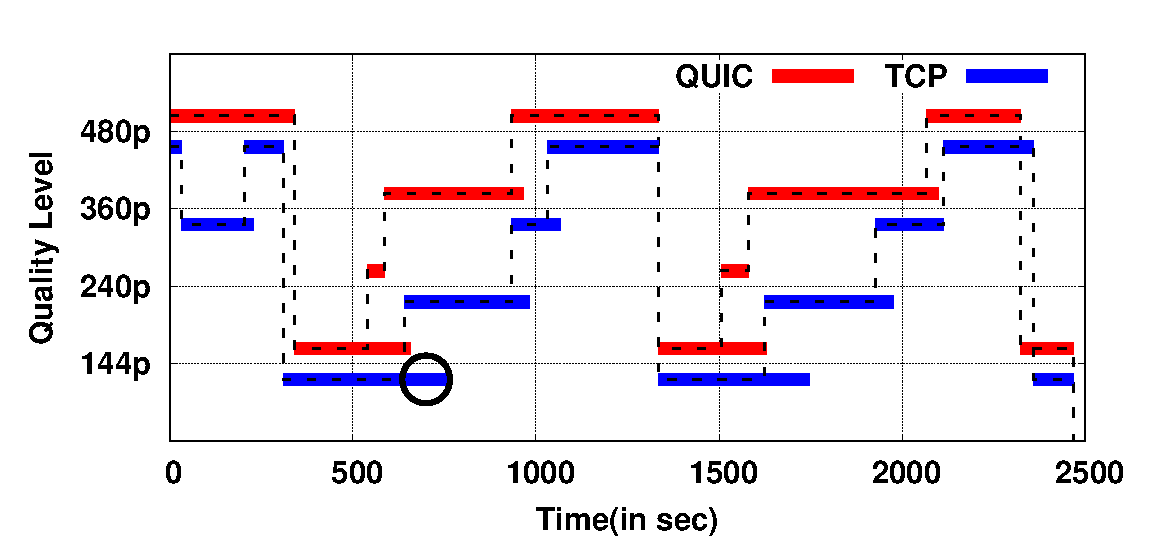
\includegraphics[width=0.7\linewidth]{img/plotdata/video/plot_timerange}
\caption{Segments downloaded at different quality levels for a YouTube video with ID $<$OJZgOOOE1zY$>$}
\label{fig:plot_timerange}
\end{figure}

Here we consider the data from a sample video with YouTube video ID $<$OJZgOOOE1zY$>$  (last accessed on 17th May, 2017) among the videos that we have downloaded during the data collection phase. \fig\ref{fig:plot_timerange} shows the downloaded segments at different video quality for this video with respect to time. 
%We plot the quality switching distribution for both the cases -- when the video was streamed through QUIC (the red line) and when the video was streamed through TCP (the blue line). 
Here we can see that there is a slight overlap between the downloaded segments of two qualities, when the streaming client upgrades the video quality from one to another. During quality upgrade, YouTube streaming client takes an restrictive approach by downloading the video segments of two different qualities simultaneously for some amount of time, so that it can revert back to the low quality immediately in case of request failure for the high quality video segment. %, in case the download request for the high quality video segment is successful. 
However, this results in data waste when the request for high quality video segment is indeed successful. 
%Next we analyze the impact of QUIC and TCP over this data wastage during adaptive streaming over the web.   

\subsubsection{Data Waste Due to Adaptive Streaming: QUIC vs TCP}
%\clearpage
%\begin{figure}[ht!]
%    \centering
%    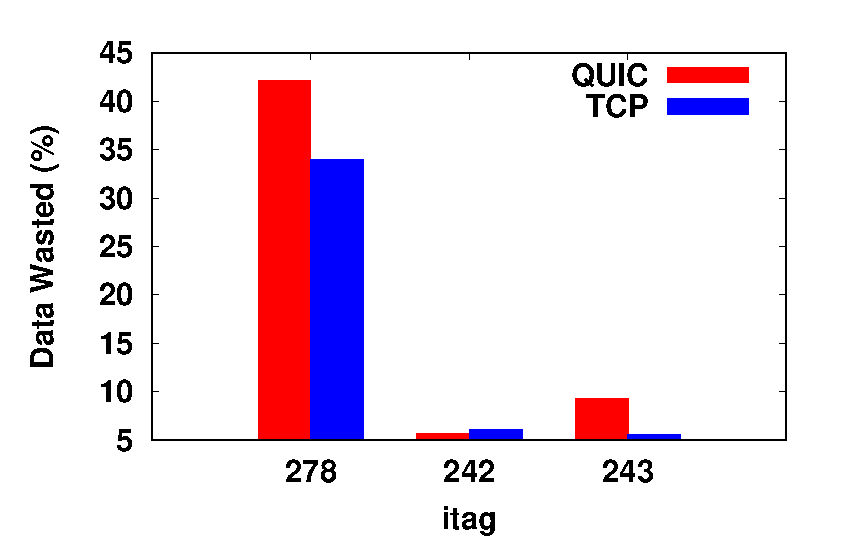
\includegraphics[width=0.9\linewidth]{img/CDF/Data_wasted_percent}
%    \caption{Amount of Data Wasted \notesc{Plot the percentage as given in the table -- then this figure is not required}\noteam{Done}}
%    \label{fig:rabuf76q1}
%\end{figure}

\begin{figure}[!t]
	\captionsetup[subfigure]{}
	\begin{center}
%		\subfloat[\label{fig:wasted_quality} At Different Quality]{
%			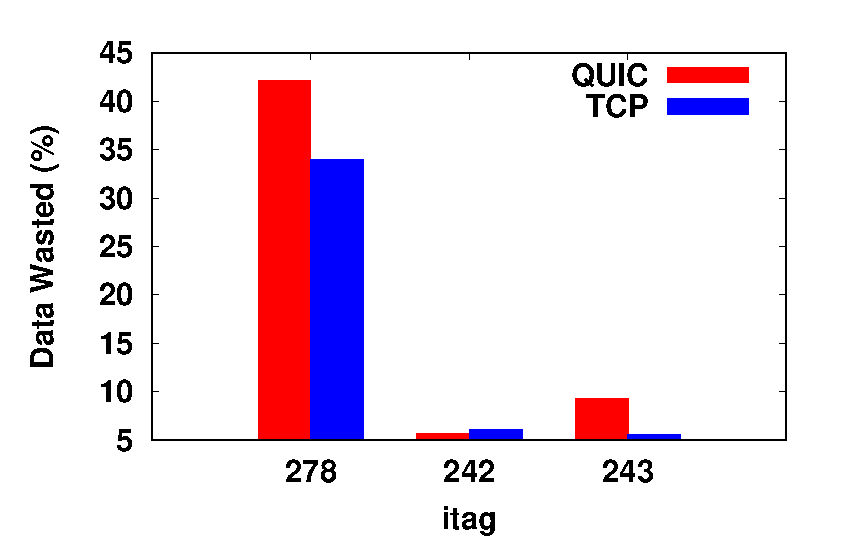
\includegraphics[width=0.48\linewidth]{img/CDF/Data_wasted_percent}
%		}
%		\subfloat[\label{fig:wasted_band}At Different Bandwidth]{
%			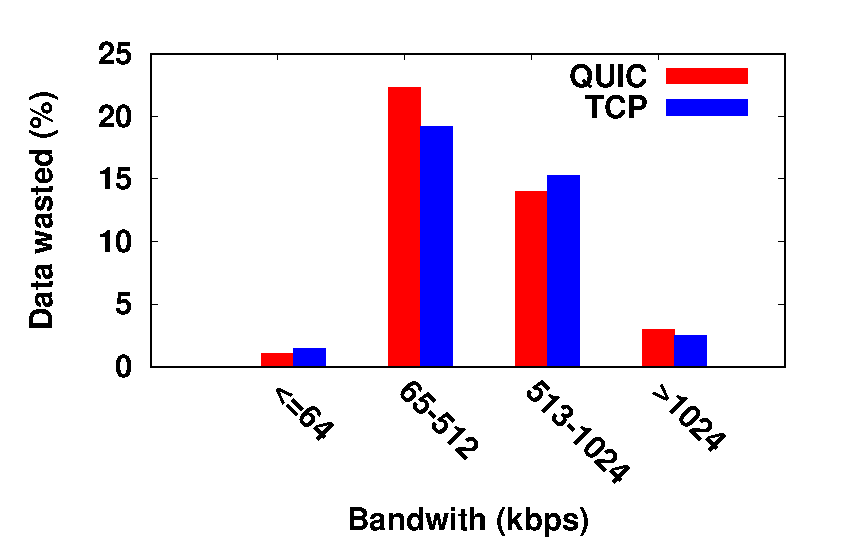
\includegraphics[width=0.48\linewidth]{img/CDF/data_wasted_bw}
%		}
        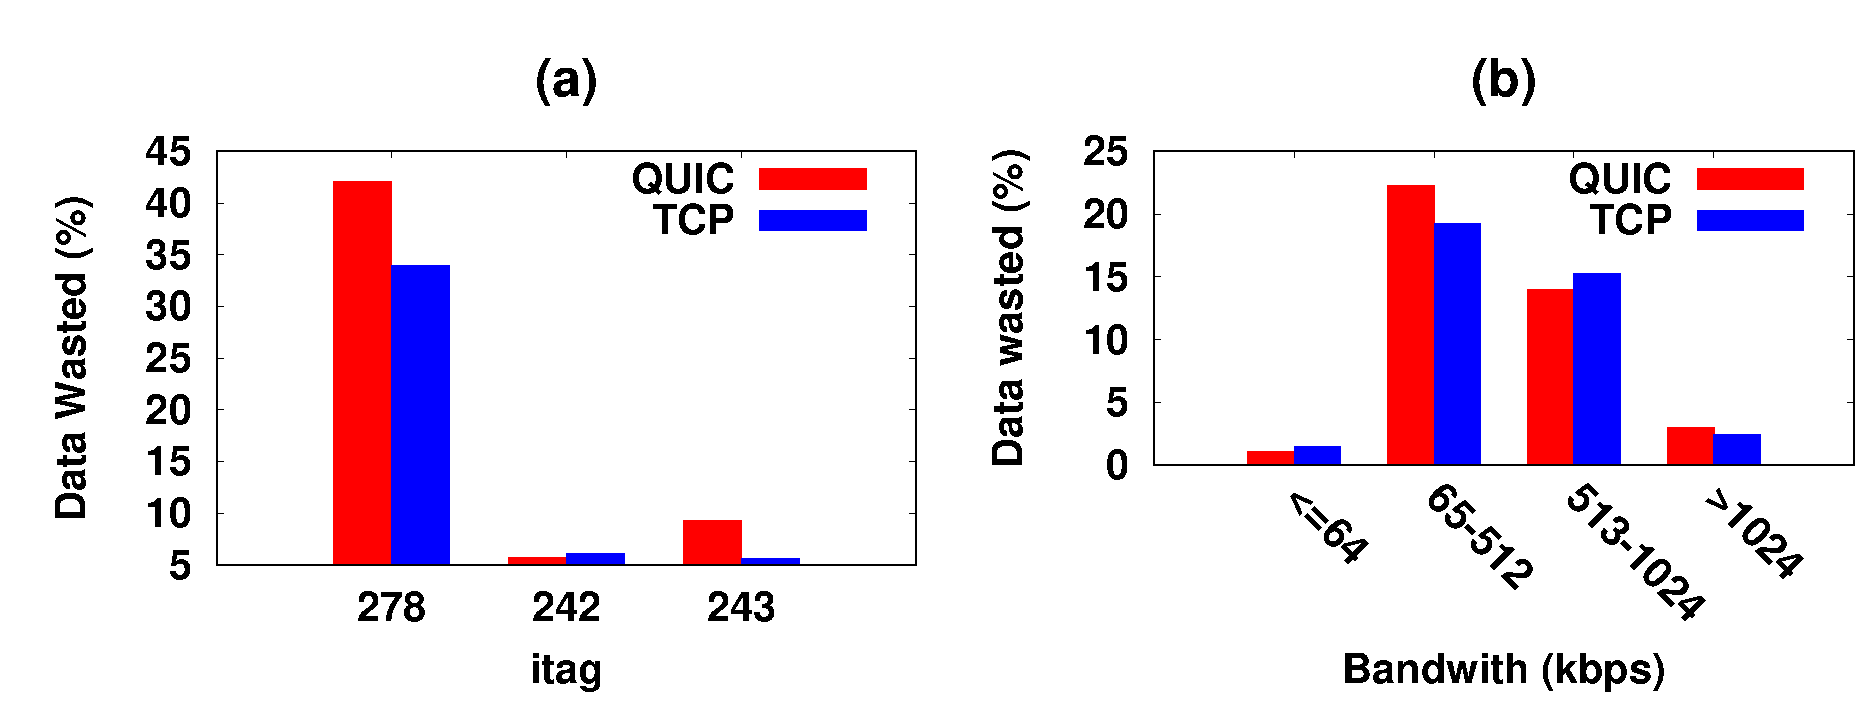
\includegraphics[width=0.9\linewidth]{img/plotdata/CDF/downloaded/data_wasted_itag_bw}
		\caption{\label{fig:data_wasted}Data wasted: (a) Different quality levels, (b) Different channel bandwidth}
	\end{center}
\end{figure}


%\notesc{Percentage of data wasted at various bandwidth buckets -- (a) $\leq 64$ Kbps, (b) $65-512$ Kbps, (c) $513-1024$ Kbps, (d) $> 1024$ Kbps}

%
%\begin{table}[ht!]
%    \centering
%    \small
%    \begin{tabular}{||c |c |c|c|c||} 
%        \hline
%        \textbf{Itag} & \textbf{Resolution} & \textbf{Downloaded}& \textbf{Wasted}& \textbf{\%}  \\ 
%        & & \textbf{(Mb)}& \textbf{(Mb)}& \textbf{Wasted}\\ 
%        \hline\hline
%        278 & 256x144 & 7669 & 3230 & 42.12\%\\ 
%        \hline
%        242 & 426x240 & 21232 & 1219 &5.74\%\\ 
%        \hline
%        243 & 640x360 & 44894 & 4187 &9.33\%\\ 
%        \hline
%        \hline
%        Total &  & 73795 & 8636 &11.7\%\\ 
%        \hline
%    \end{tabular}
%    \caption{Data Wastage for QUIC}
%    \label{table:3}
%\end{table}

%\begin{table}[ht!]
%    \centering
%%    \scriptsize
%    \small
%    \begin{tabular}{||c |c |c|c|c||} 
%        \hline
%        \textbf{Itag} & \textbf{Resolution} & \textbf{Downloaded}& \textbf{Wasted}& \textbf{\%}  \\
%        & & \textbf{(Mb)}& \textbf{(Mb)}& \textbf{Wasted }  \\
%        \hline\hline
%        278 & 256x144 & 10049 & 3412 & 33.95\%\\ 
%        \hline
%        242 & 426x240 & 23028 & 1399 &6.07\%\\ 
%        \hline
%        243 & 640x360 & 37911 & 2134 &5.63\%\\ 
%        \hline
%        \hline
%        Total &  & 70988 & 6945 &9.78\%\\ 
%        \hline
%    \end{tabular}
%    \caption{Data Wastage for TCP}
%    \label{table:4}
%\end{table}
\begin{figure*}[!t]
	\captionsetup[subfigure]{}
	\begin{center}
		%		\subfloat[\label{fig:plot_itag_pdf_bucket1}Bandwidth $\leq 64$ Kbps]{
		%			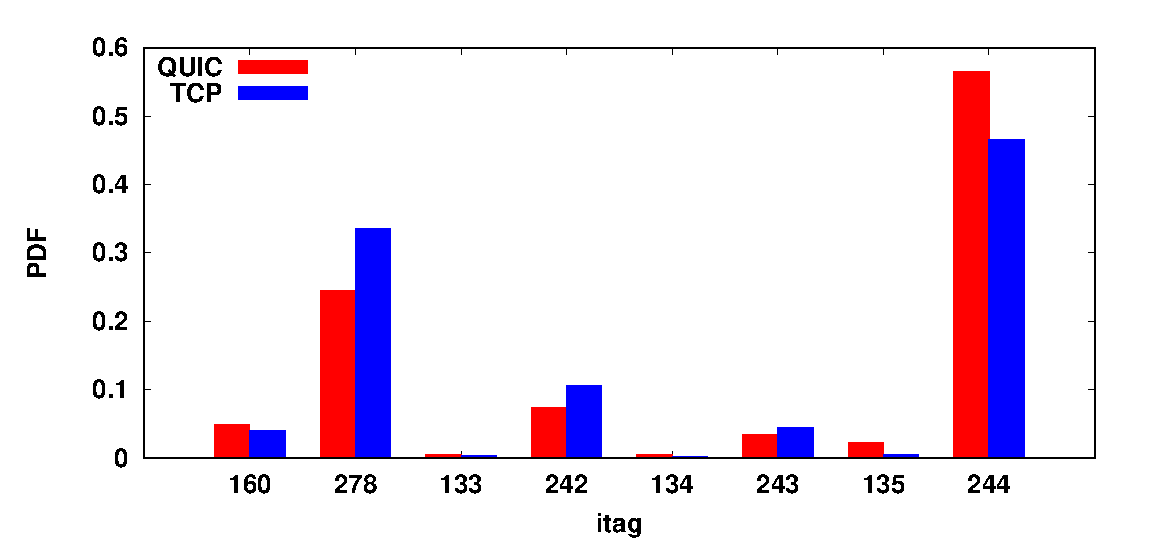
\includegraphics[width=0.32\linewidth]{img/PDF/plot_itag_pdf_bucket1}
		%		}
		%		\subfloat[\label{fig:plot_itag_pdf_bucket2} $64$ Kbps $<$ Bandwidth $ \leq 1024$ Kbps]{
		%			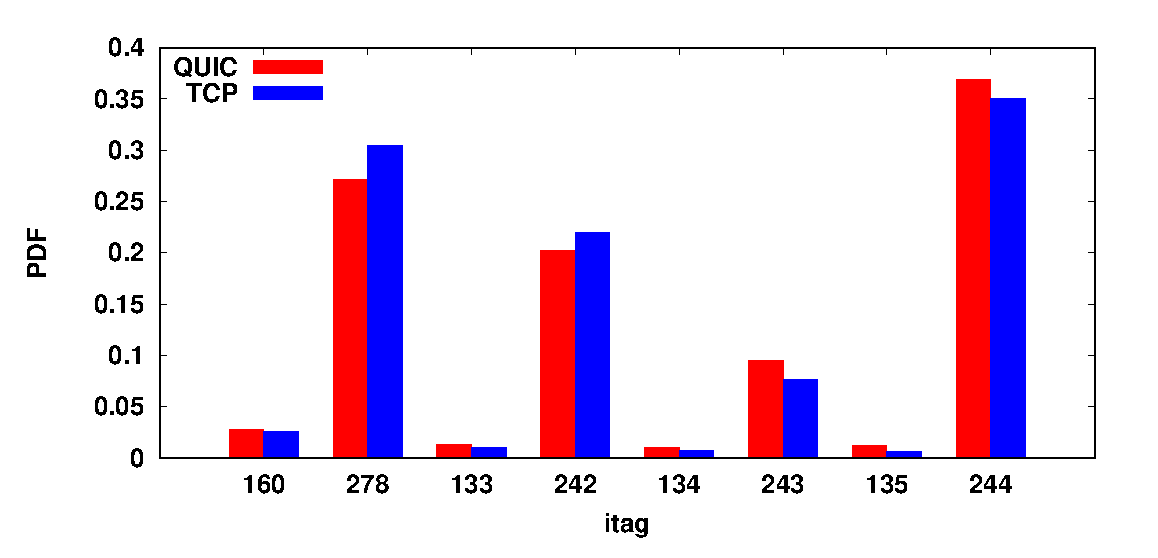
\includegraphics[width=0.32\linewidth]{img/PDF/plot_itag_pdf_bucket2}
		%		}
		%		\subfloat[\label{fig:plot_itag_pdf_bucket3}Bandwidth  $> 1024$ Kbps]{
		%			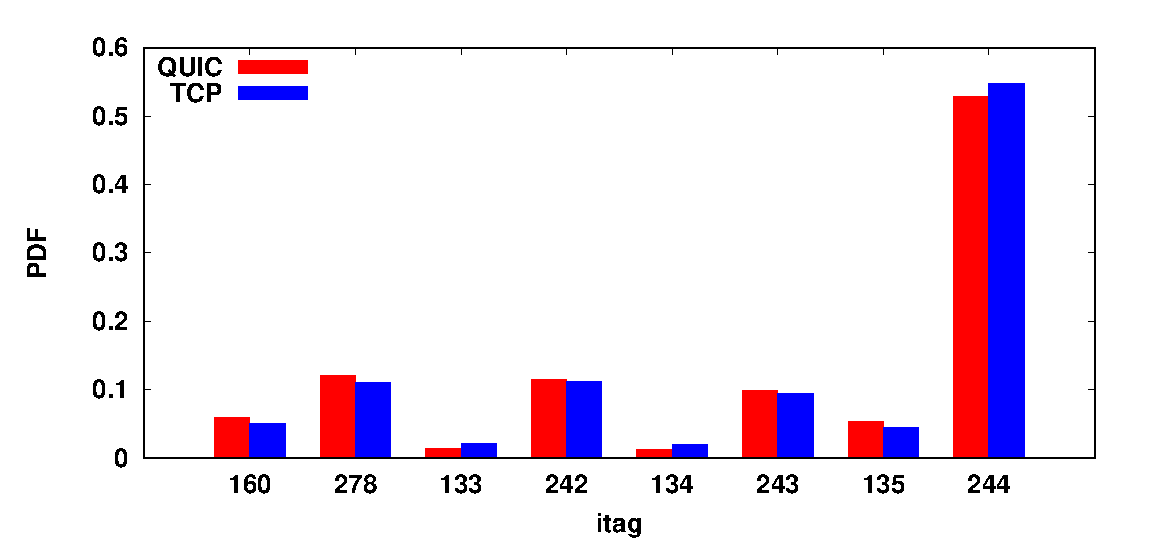
\includegraphics[width=0.32\linewidth]{img/PDF/plot_itag_pdf_bucket3}
		%		}
		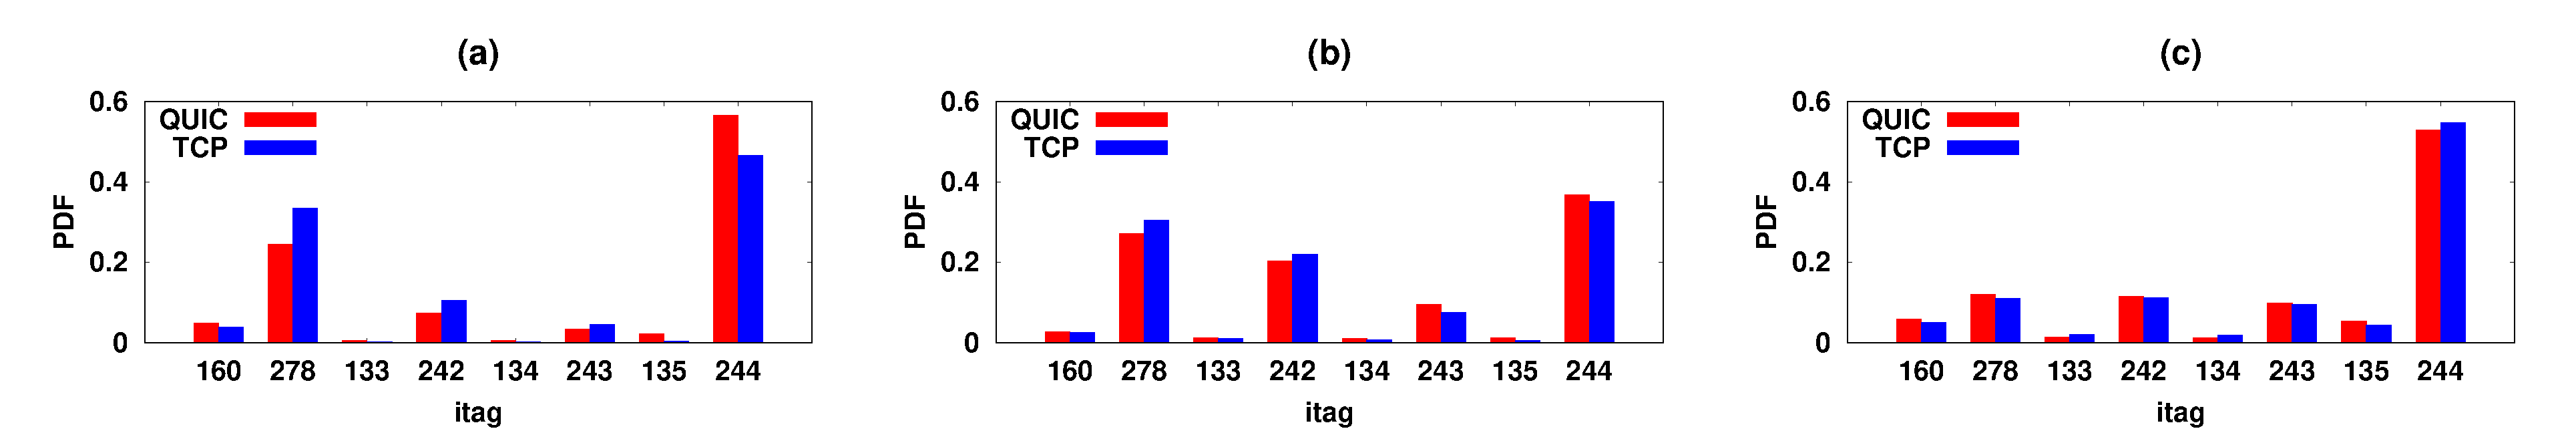
\includegraphics[width=0.8\linewidth]{img/plotdata/PDF/itag/plot_itag_pdf_bucket123}
		\caption{\label{fig:quality_change}Change for quality levels at different bandwidth: (a) $\leq 64$ Kbps, (b)  between $64$ and $1024$ Kbps, (c) $> 1024$ Kbps}
	\end{center}
\end{figure*}

\fig\ref{fig:data_wasted} compares \ac{QUIC} enabled streaming and \ac{TCP} enabled streaming in terms of percentage of data waste during quality upgrades. 
%Here we show the percentage data waste (percentage of total downloaded data that has not been played during the video rendering) for different quality levels, when the YouTube client switches the quality from this level to a higher level. 
We observe that data waste with \ac{QUIC} is more compared to \ac{TCP}. Further, data waste is comparatively high when the available bandwidth is less that $512$ Kbps (\fig\ref{fig:data_wasted}(b)). 
%It can be noted that frequent quality switching increases the amount of data wastage. 
By observing data logs, we have found that for \ac{QUIC} enabled streaming, the YouTube client tries to make more number of quality upgrade attempts at the low bandwidth, which are not successful. 
%In the next subsection, we give a detailed analysis of this behavior. 
Consequently, \ac{QUIC} results in more data waste. In the next section, we give a detailed view of this. 
%\fig\ref{fig:wasted_band} plots the percentage data wasted for different network conditions measured in terms of available channel bandwidth. We observe that 
%Further, 
%This supports our hypothesis that the quality upgrade attempts at low bandwidth under QUIC is not stable that results in comparatively high data wastage. In the next section, we discuss additional results in support of this hypothesis and to analyze the video streaming behavior of QUIC and TCP under different channel conditions. 


%\subsection{Comparison of Streaming data rate between QUIC and TCP}
%In this section we will examine whether the streaming data rate variation  whenever the bandwidth changes, is similar in QUIC and TCP. To compare the behavior of streaming data rate adaptation, we plot how the requested video segment length (specified by the \textit{range} parameter) per video playback request, changes with change in link bandwidth in \fig\ref{fig:rser1}. For this, we convert the byte range mentioned in the video playback request to the equivalent video playback time, and find out the video segment length in terms of playback time. Whenever the link bandwidth increases, YouTube first increases the segment length of lower quality video and buffers maximum amount of video data. It then switches to the higher quality video but with smaller segment lengths. At this point, we observe an overlap between the segments of two different video qualities. It then progressively increases the segment length and repeats the procedure for the next higher quality level video if the link quality improves further (measured through the increase rate of \textit{rbuf}). However, when the link quality drops, in a similar way, YouTube first starts requesting for same quality video chunks of smaller segments, and drops the segment length. If it still observes a drop in \textit{rbuf} after reducing the segment length in the playback requests, then it switches to request for the next lower quality level video chunks of smaller segments. If the \textit{rbuf} becomes stable, then only it again increases the segment length. This behaviour is similar to both QUIC and TCP over YouTube but from the plots we can observe that QUIC is able to switch to higher quality from a lower quality in a shorter interval of time when compared to TCP. 
%
%
%%\newpage
%%\begin{figure}[!ht] 
%%    \centering
%%    \begin{minipage}{0.45\linewidth}
%%        \includegraphics[width=\linewidth]{img/QUICPlots/plot_sengmentLength} 
%%        \caption{QUIC}
%%        \label{fig:seg1Q}
%%    \end{minipage}
%%    \begin{minipage}{0.45\linewidth}
%%        \includegraphics[width=\linewidth]{img/TCPPlots/plot_sengmentLength}
%%        \caption{TCP}
%%        \label{fig:rseg1T}
%%    \end{minipage} 
%%    \caption{Plot for \textit{Segment Length} over time for a YouTube video of id $<$OJZgOOOE1zY$>$}
%%    \label{fig:rser1}
%%\end{figure}
%\begin{figure}[!t]
%    \captionsetup[subfigure]{}
%    \begin{center}
%        \subfloat[\label{fig:seg1Q}QUIC]{
%            \includegraphics[width=0.48\linewidth]{img/QUICPlots/plot_sengmentLength}
%        }
%        \subfloat[\label{fig:rseg1T}TCP]{
%            \includegraphics[width=0.48\linewidth]{img/TCPPlots/plot_sengmentLength}
%        }
%        
%        \caption{\label{fig:rser1}Plot for \textit{Segment Length} over time for a YouTube video of id $<$OJZgOOOE1zY$>$}
%    \end{center}
%\end{figure}
%%\clearpage
%
%%\section{Comparison of Video Quality observed over time between QUIC and TCP}
%From \fig\ref{fig:rser1}, we observe that as link quality increases, \textit{rbuf} also increases, and YouTube client progressively makes requests for higher \textit{itag} values. Further, whenever the value of \textit{rbuf} drops, YouTube client switches \textit{itag} requests for a lower video quality. We already know that YouTube video quality adaptation algorithm is based on the client’s observation of the change in receive buffer – a sharp increase in received buffer gives an indication for fetching data of higher video quality, whereas YouTube takes a conservative approach of requesting data for lower video quality whenever the client observes a sharp drop in receive buffer size.
%
%From the earlier discussion, we know that \textit{range} parameter gives the byte range of the video streaming data for which the client sent a request to the server. We first convert this range parameter to equivalent video segment length in terms of video playback time. This can be done by looking into the video file header that provides a mapping between the byte range and playback time. We use the Python package {\fontfamily{qcr}\selectfont python-ebml} to extract such information from the video files. The figures in \fig\ref{fig:rserr1} plots the video segments (in terms of video playback time, as shown in Xaxis) and the corresponding \textit{itag} values for which the client makes a request. YouTube takes an opportunistic approach for downloading higher quality video segments when the link quality improves, but takes a conservative approach when the link quality drops. In the opportunistic approach, it downloads the video chunks of both the video qualities in parallel, whenever it decides to switch from the lower quality to the higher quality. However, in the conservative approach, it directly sends the request for lower quality video when the link quality drops. That is why we notice an an overlap between the segments of lower quality and higher quality when the video quality improves.
%
%When we observe the plot for a single video (\fig\ref{fig:rser1} and \fig\ref{fig:rserr1}), we can see that there are overlaps between the segment downloaded. So, there is some data wastage is happening. In next section, we compare data wastages during video playback using the normal TCP and the QUIC.
%
%%When we observe the plot for a single video (\fig\ref{fig:rserr1}), it is evident that QUIC is able to maintain video quality that is higher or same as that of TCP in most cases. From these three plots (\noteam{I could not figure out which three.}) we can expect that DASH will perform better when QUIC is employed as transport layer protocol rather than TCP in terms of video quality. In order to prove the above hypothesis we will show the Cumulative Distribute Function graphs collected over 175 videos in the next section.
%
%%\begin{figure}[!ht] 
%%    \centering
%%    \begin{minipage}{0.45\linewidth}
%%        \includegraphics[width=\linewidth]{img/QUICPlots/plot_timerange} 
%%        \caption{QUIC}
%%        \label{fig:rseg1Q}
%%    \end{minipage}
%%    \begin{minipage}{0.45\linewidth}
%%        \includegraphics[width=\linewidth]{img/TCPPlots/plot_timerange}
%%        \caption{TCP}
%%        \label{fig:rsegr1T}
%%    \end{minipage} 
%%    \caption{Plot for time range of different qualities for a YouTube video of id $<$OJZgOOOE1zY$>$}
%%    \label{fig:rserr1}
%%\end{figure}
%
%\begin{figure}[!t]
%    \captionsetup[subfigure]{}
%    \begin{center}
%        \subfloat[\label{fig:rseg1Q}QUIC]{
%            \includegraphics[width=0.48\linewidth]{img/QUICPlots/plot_timerange}
%        }
%        \subfloat[\label{fig:rsegr1T}TCP]{
%            \includegraphics[width=0.48\linewidth]{img/TCPPlots/plot_timerange}
%        }
%        
%        \caption{\label{fig:rserr1}Plot for \textit{Time Range} over time for a YouTube video of id $<$OJZgOOOE1zY$>$}
%    \end{center}
%\end{figure}
%%\clearpage


\subsection{Impact of Channel Bandwidth over Video Streaming: QUIC vs TCP}
From the previous discussion and analysis, we have observed that the performance of video streaming over \ac{QUIC} has a dependency over the available channel bandwidth. 
%The data wastage due to YouTube adaptive streaming is more when channel bandwidth is low. To explore this behavior further, we next analyze the adaptive streaming behavior over QUIC under different channel conditions measured in terms of available channel bandwidth. 
Here, we particularly look the evolution of three parameters at different available bandwidth, which control the adaptive streaming behavior -- (a) quality switching (using \textit{itag}), (b) buffer occupancy at the YouTube streaming client (using \textit{rbuf}) and (c) segment length adaptation during streaming (using \textit{range} ). We consider three channel conditions -- (a) poor (available bandwidth is less than $64$ Kbps), (b) medium (available bandwidth is in between $64$ Kbps and $1$ Mbps), and (c) good (available bandwidth is more than $1$ Mbps).

\subsubsection{Video Quality Adaptation}
%For a particular bandwidth level we counted the number of requests made for each \textit{itag} and from that we calculated the probability for an  \textit{itag} as the number of requests made for that itag divided by total number of requests made.
%
%\begin{figure}[!ht]
%    \centering
%    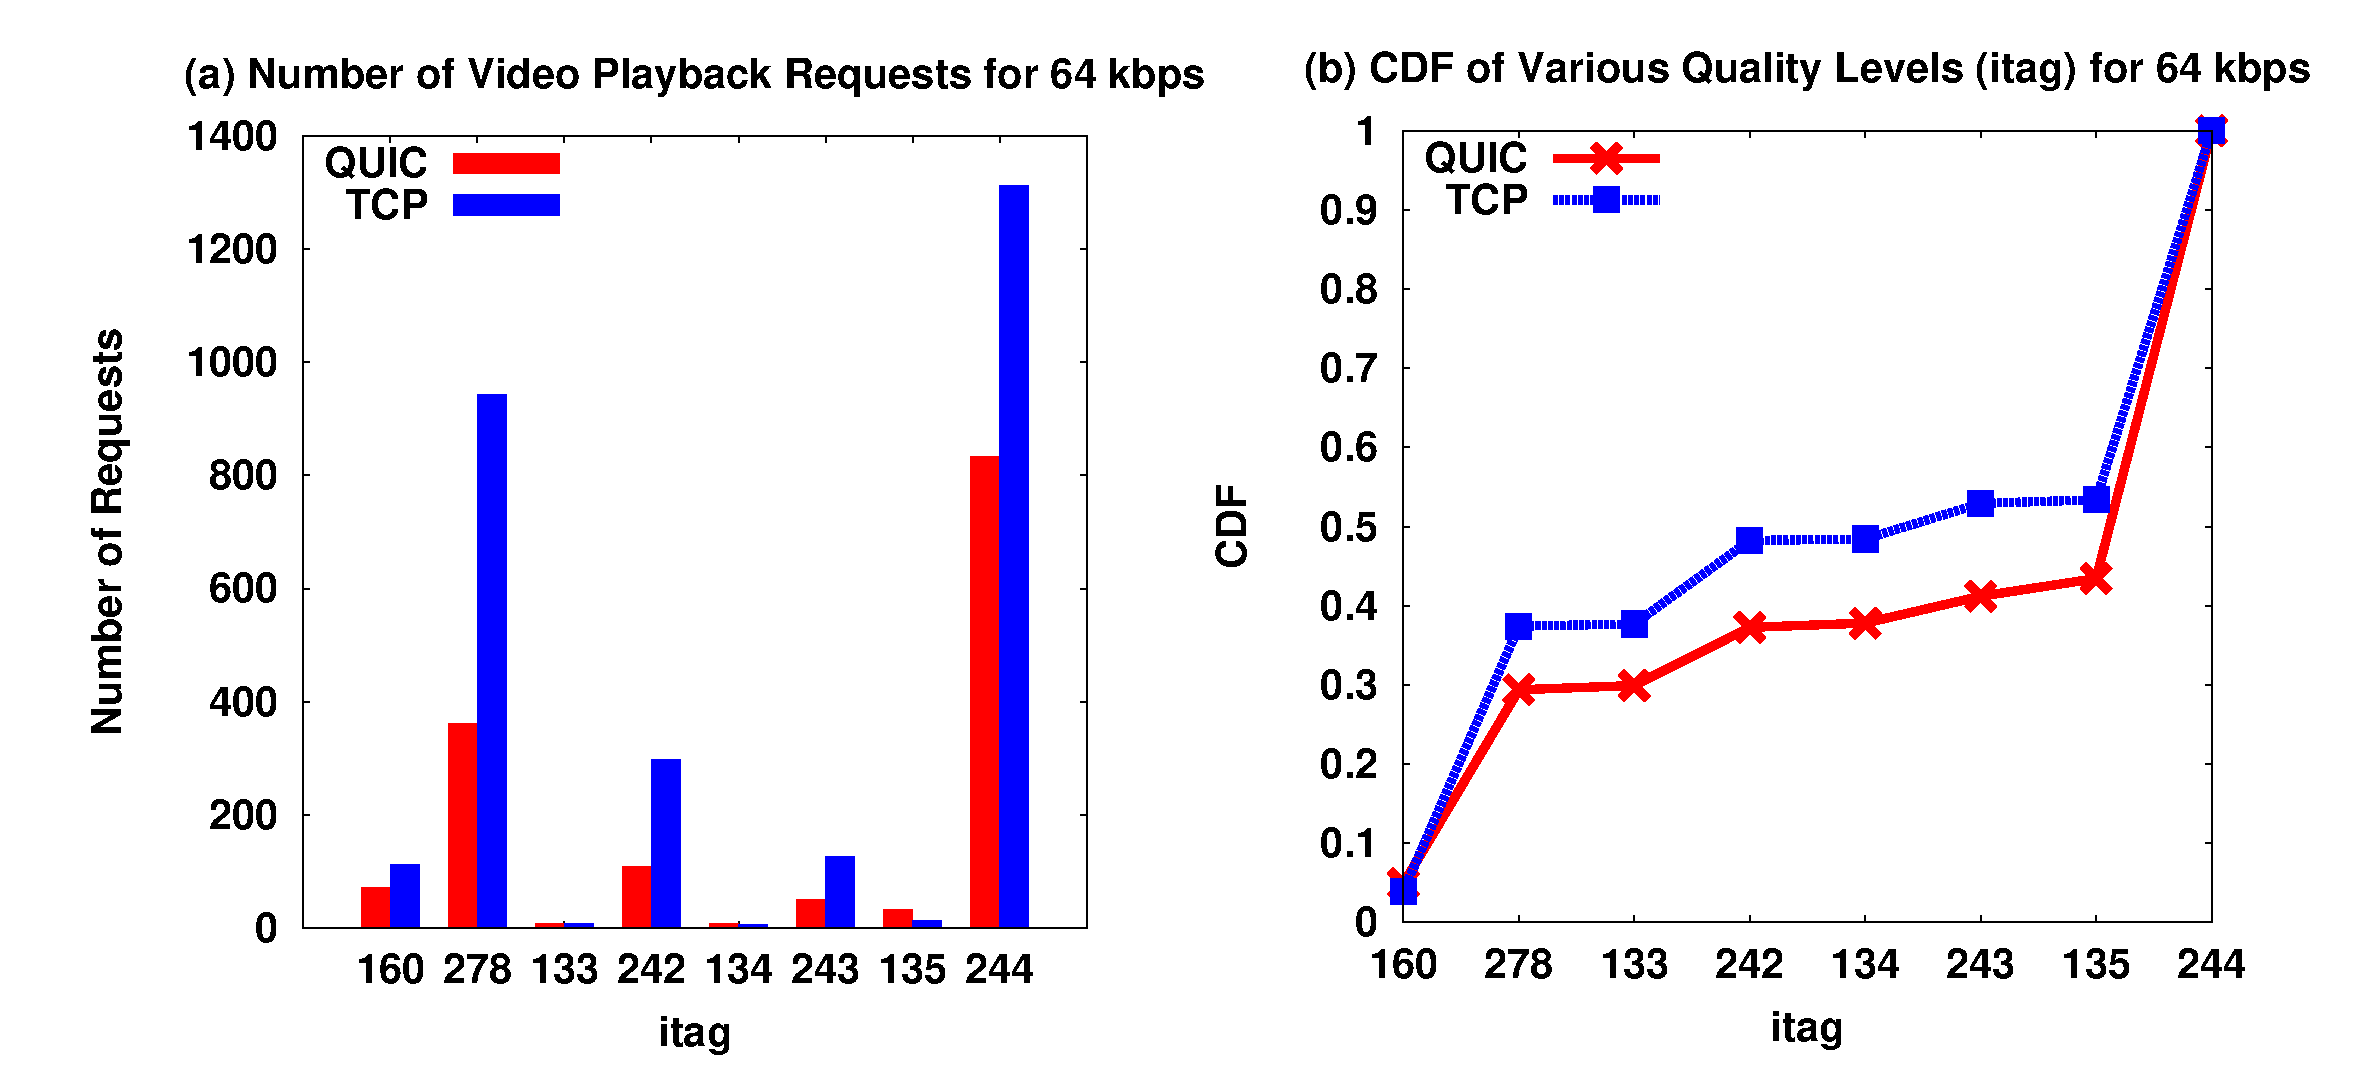
\includegraphics[width=\linewidth]{img/CDF/plot_itag_65536}
%    \caption{Number of requests and CDF of itag at 64 kbps}
%    \label{fig:itag6556}
%\end{figure}
%
%\begin{figure}[!ht]
%    \centering
%    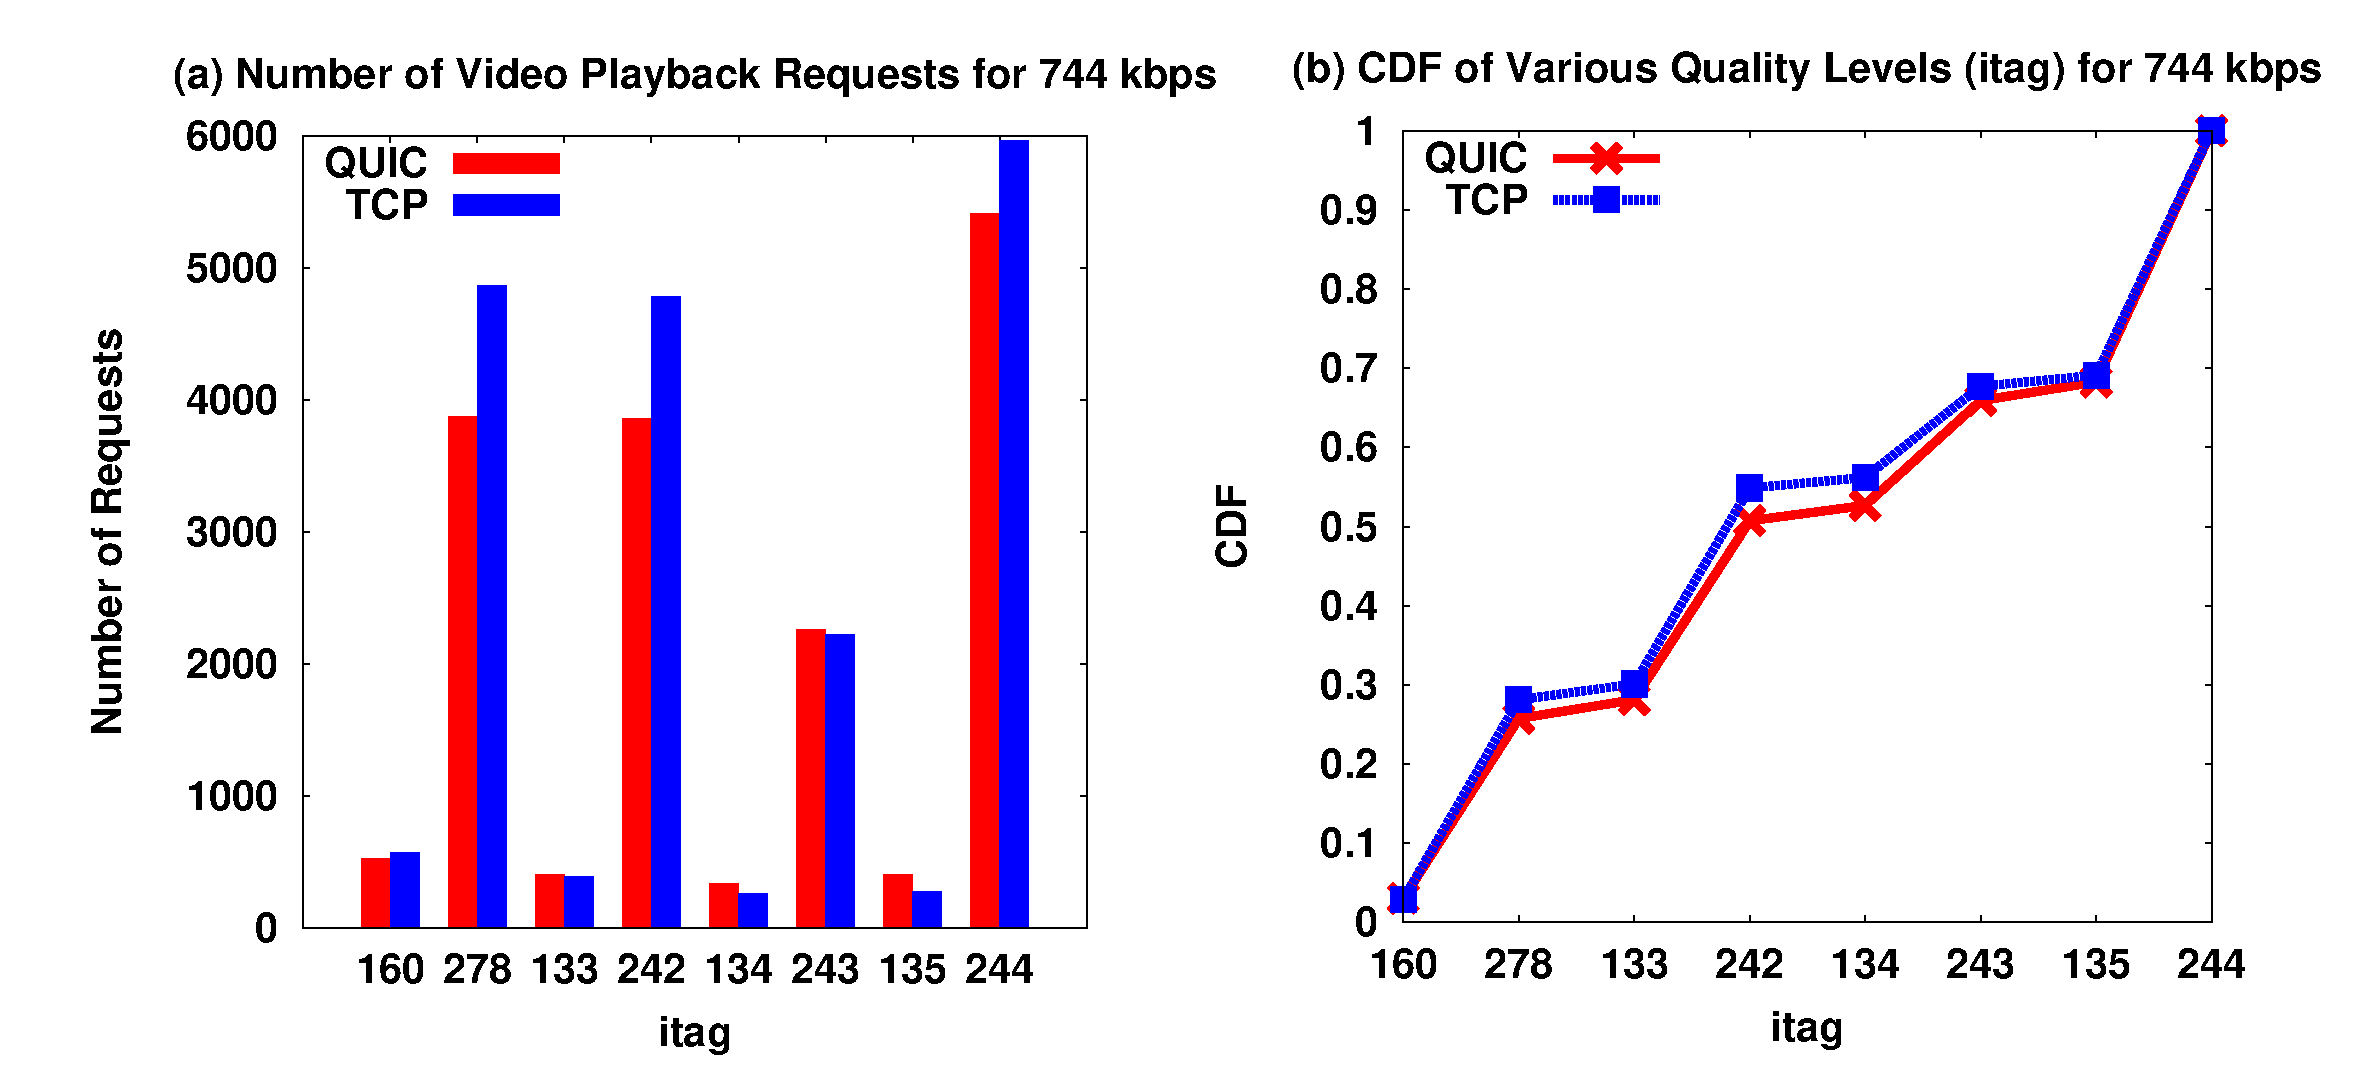
\includegraphics[width=\linewidth]{img/CDF/plot_itag_761856}
%    \caption{Number of requests and CDF of itag at 744 kbps}
%    \label{fig:itag761}
%\end{figure}
%
%
%
%\begin{figure}[h]
%    \centering
%    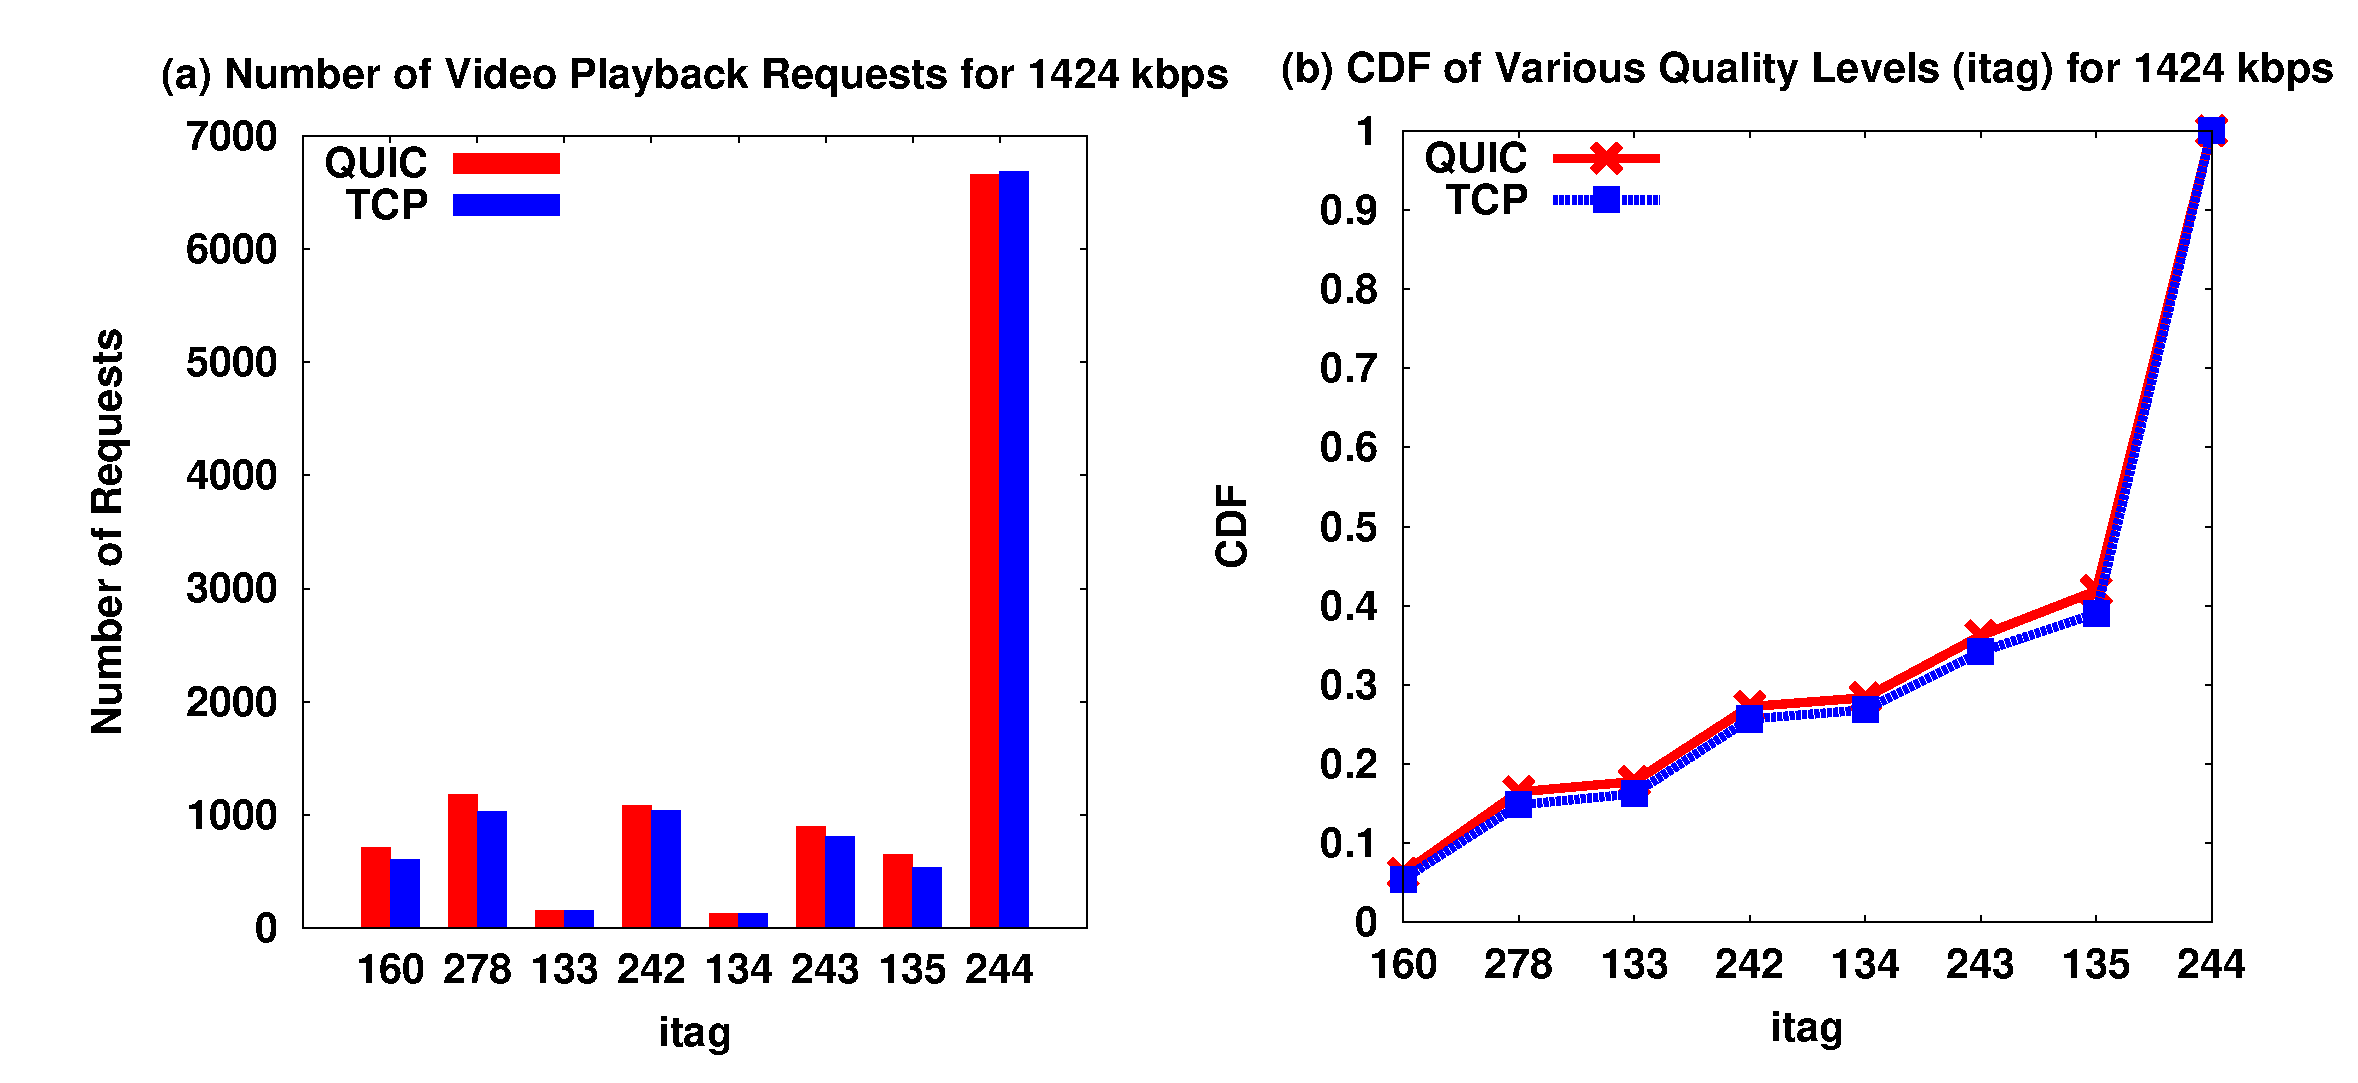
\includegraphics[width=\linewidth]{img/CDF/plot_itag_1458176}
%    \caption{Number of requests and CDF of itag at 1424 kbps}
%    \label{fig:itag76111}
%\end{figure}




We compute the \ac{PDF} for various \textit{itag} values during the video bitrate adaption procedure, as shown in \fig\ref{fig:quality_change}. 
%\begin{addmargin}[2.1cm]{2.1cm}
We observe that at poor bandwidth, \ac{QUIC} has higher tendency than \ac{TCP} towards high quality videos, but as the bandwidth increases, both \ac{QUIC} and \ac{TCP} show similar tendencies towards video quality adaptation. So, \ac{QUIC} may improve the viewing performance with a better video quality than \ac{TCP}  at poor channel connection. However, as we observed, many of these quality upgrades are not very stable, and this frequent quality upgrades result in more data waste, as we observed earlier. 
%At lower speeds QUIC does not make as many requests to the server as TCP makes but at higher speeds both the protocols makes the same number of requests. This implies that QUIC is more aware of the network conditions than TCP. In the above plots when the bandwidth is at 64Kbps TCP has made almost twice the number of requests as QUIC made. This is because at 64Kbps when almost all the packets are dropped, TCP unable to quickly recognize the change in bandwidth makes the request for the same higher itag value and when they fail it makes requests for lower itags. For the total set of 175 videos the number of requests made by QUIC are lesser in number when compared to TCP which implies that QUIC requires less number of requests to serve the same or higher quality data.
%\end{addmargin}
%\restoregeometry

\subsubsection{Buffering at the Playback Client}

\begin{figure}[!t]
	\captionsetup[subfigure]{}
	\begin{center}
%		\subfloat[\label{fig:rbuf_bucket1}Bandwidth $ \leq 64 $ Kbps]{
%			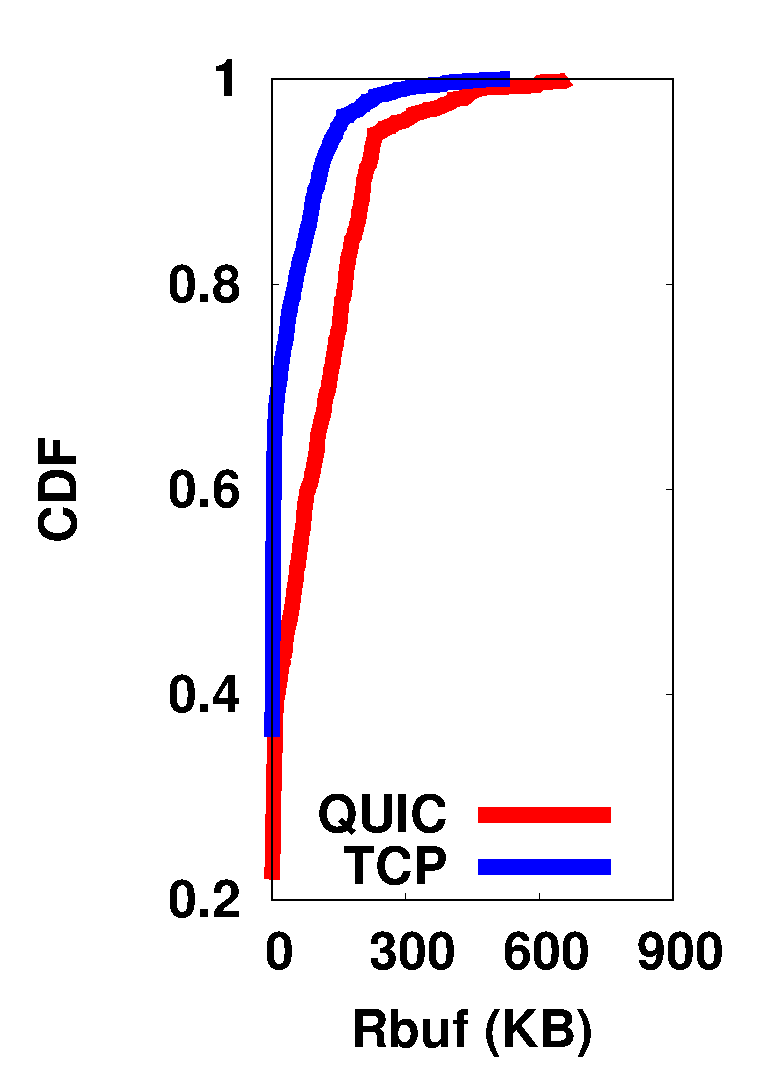
\includegraphics[width=0.32\linewidth]{img/CDF/plot_rbuf_bucket1}
%		}
%		\subfloat[\label{fig:rbuf_bucket2} $64$ Kbps $<$ Bandwidth $ \leq 1024$ Kbps]{
%			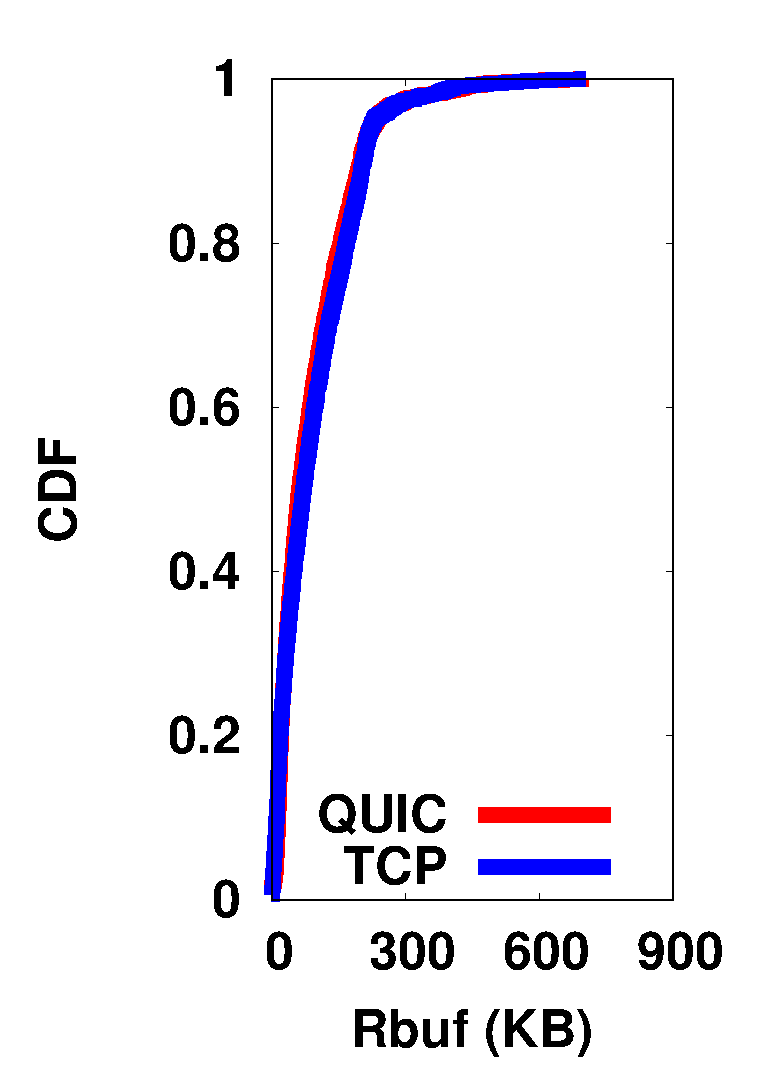
\includegraphics[width=0.32\linewidth]{img/CDF/plot_rbuf_bucket2}
%		}
%		\subfloat[\label{fig:rbuf_bucket3}Bandwidth  $> 1024$ Kbps]{
%			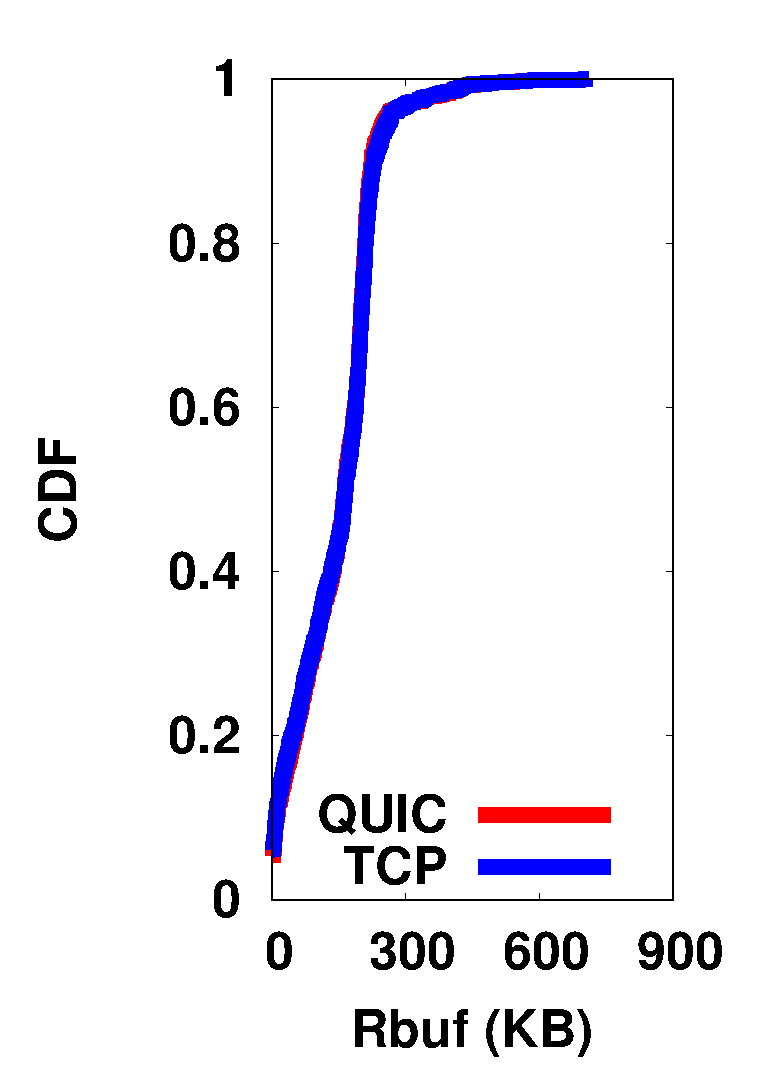
\includegraphics[width=0.32\linewidth]{img/CDF/plot_rbuf_bucket3}
%		}
        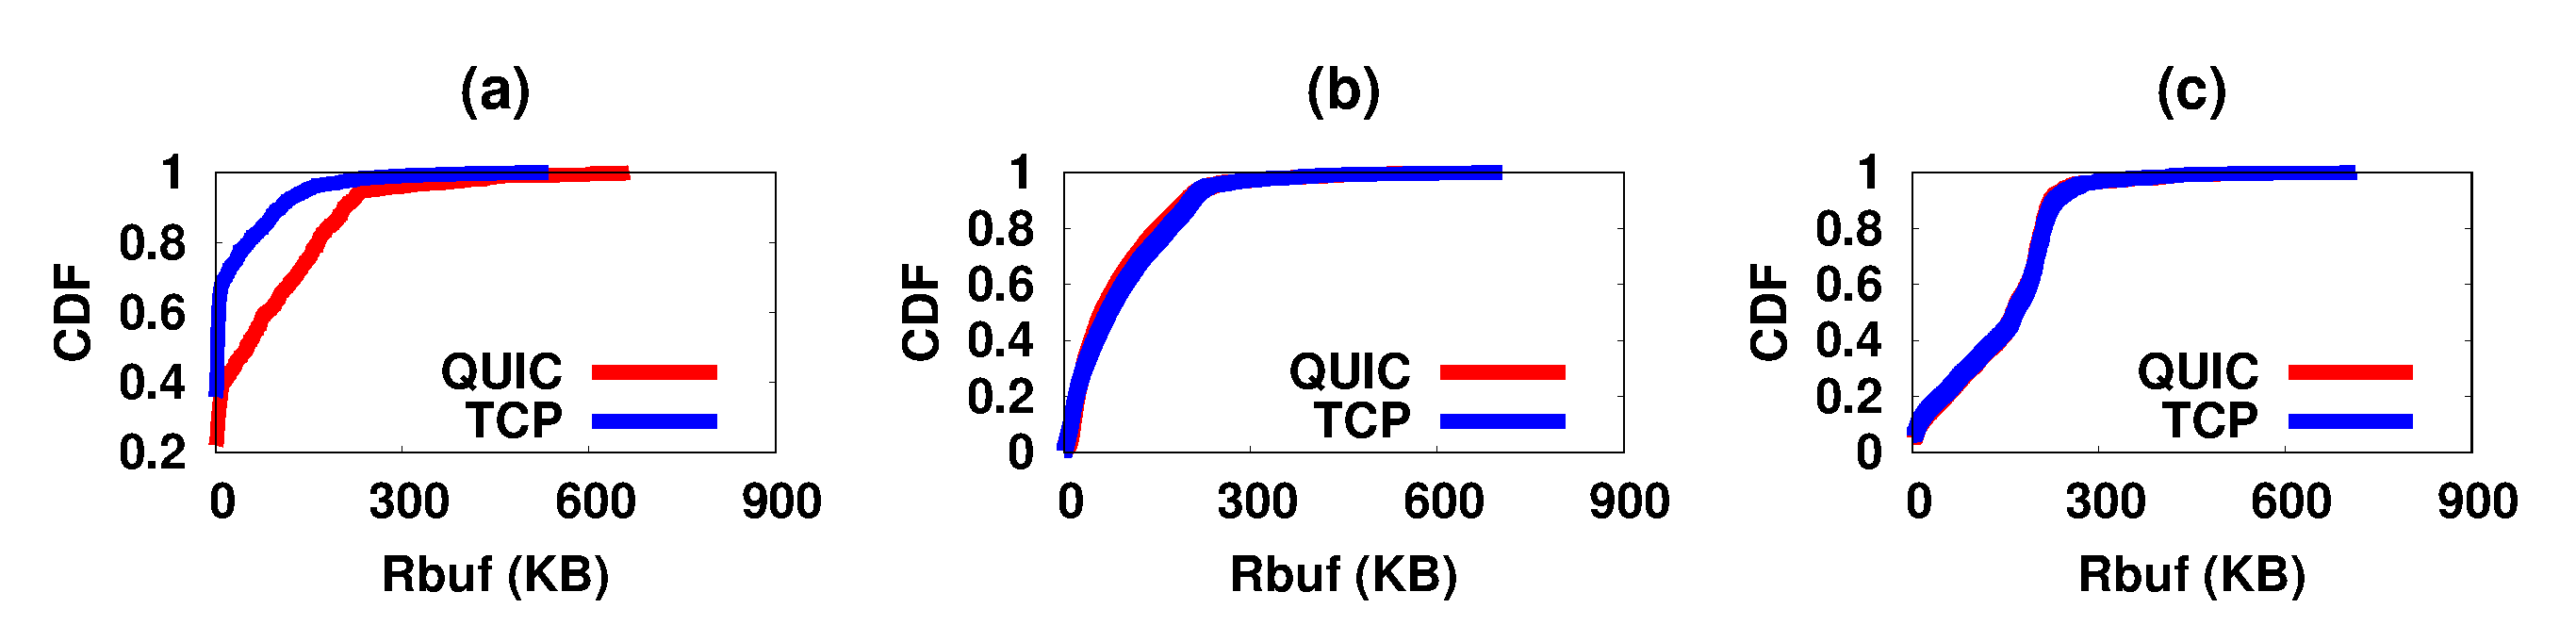
\includegraphics[width=\linewidth]{img/plotdata/CDF/Rbuf/plot_rbuf_bucket123}
		\caption{\label{fig:rbuf}Client buffer occupancy with respect to various bandwidth levels: (a) $\leq 64$ Kbps, (b)  between $64$ and $1024$ Kbps, (c) $> 1024$ Kbps}
	\end{center}
\end{figure}


\fig\ref{fig:rbuf} shows playback buffer occupancy distribution at the YouTube client in terms of \ac{CDF} for various \textit{rbuf} values extracted from the playback requests. We observe that at high bandwidth, there is not much difference between \ac{TCP} and \ac{QUIC} in terms of playback buffer occupancy. However, at low bandwidth, \ac{QUIC} fills up the playback buffer faster than \ac{TCP}, resulting in higher values of \textit{rbuf}. 
%has higher tendency towards higher \textit{rbuf} values when compared to TCP, indicating that QUIC tries to fill the client buffer fast even when the bandwidth is low. 
YouTube uses playback buffer occupancy as a feedback for video quality adaptation~\cite{mondal2017youtube,krishnappa2013dashing}
% -- if the buffer fills fast, the adaptive streaming client assumes the channel quality to be good, and switches to a high quality level for next video segment requests. However, as we have observed earlier, 
This sometime triggers a unsuccessful quality upgrade request for \ac{QUIC} enabled streaming, as the actual channel quality may not be suitable for high bitrate video streaming. This results in large number of rebuffering (\fig\ref{fig:bitrate_rebuffering}(b)) and comparatively high data waste (\fig\ref{fig:data_wasted}).

%This majorly implies that the chance for buffering is lower for QUIC when compared to TCP as buffering mainly occurs at poor Internet speeds supporting the statement made by Google that there were fewer rebuffers when QUIC is used instead of TCP.


%\notesc{Merge the three plots in a single plot -- (a) Bandwidth $ \leq 64 $ Kbps, (b) $64$ Kbps $<$ Bandwidth $ \leq 1024$ Kbps, (c) Bandwidth  $> 1024$ Kbps} \noteam{Done. \fig\ref{fig:rbuf}}
\begin{comment}
\begin{figure}[!ht]
    \centering
    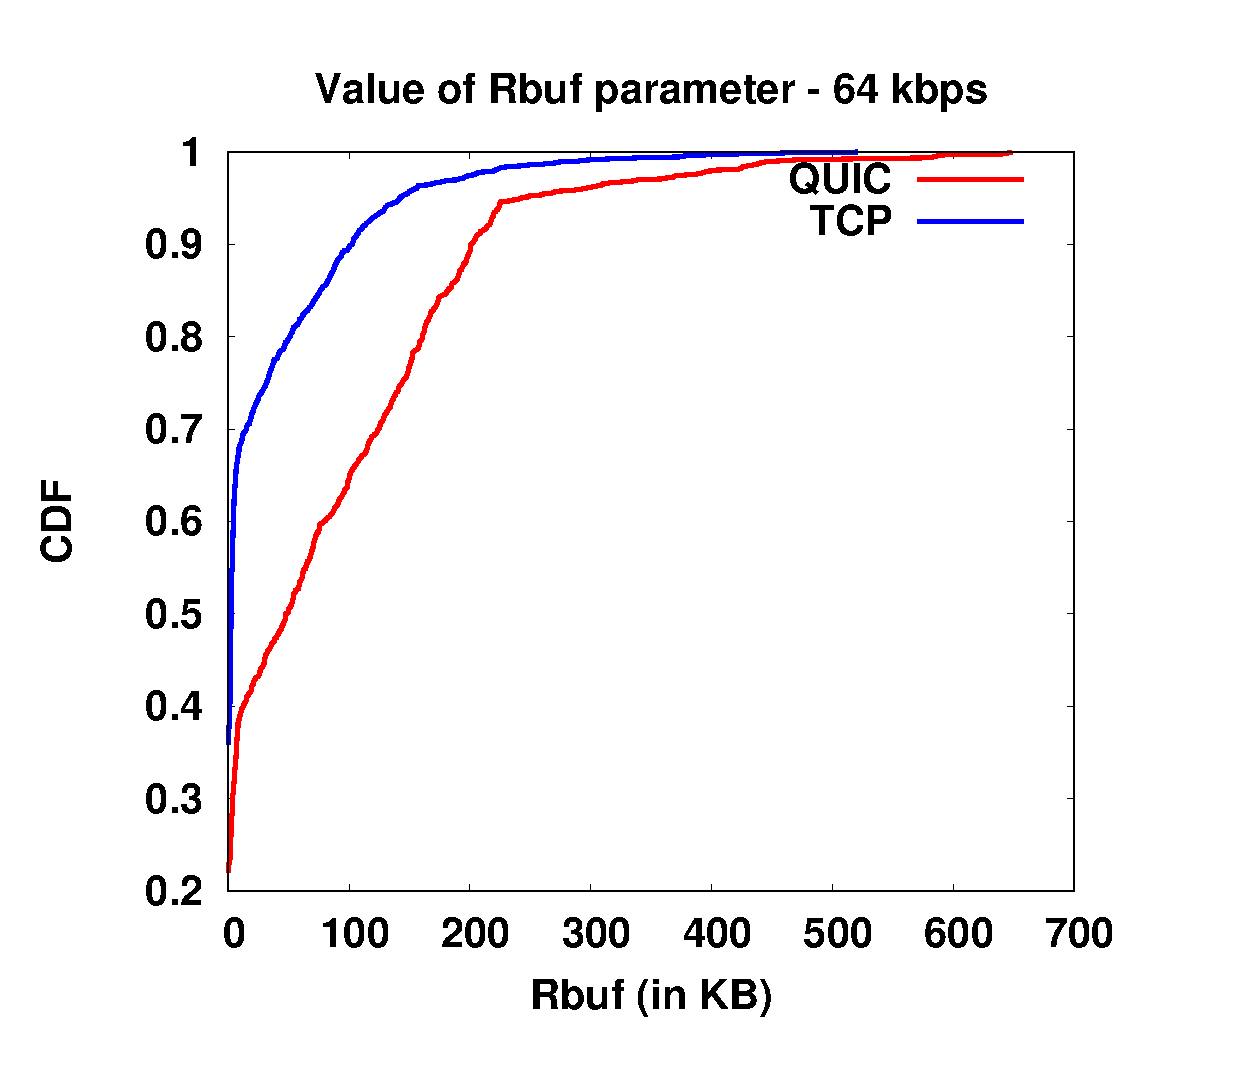
\includegraphics[width=0.9\linewidth]{img/CDF/plot_rbuf_65536}
    \caption{CDF of rbuf at 64 kbps}
    \label{fig:rbuf6556}
\end{figure}

\begin{figure}[!ht]
    \centering
    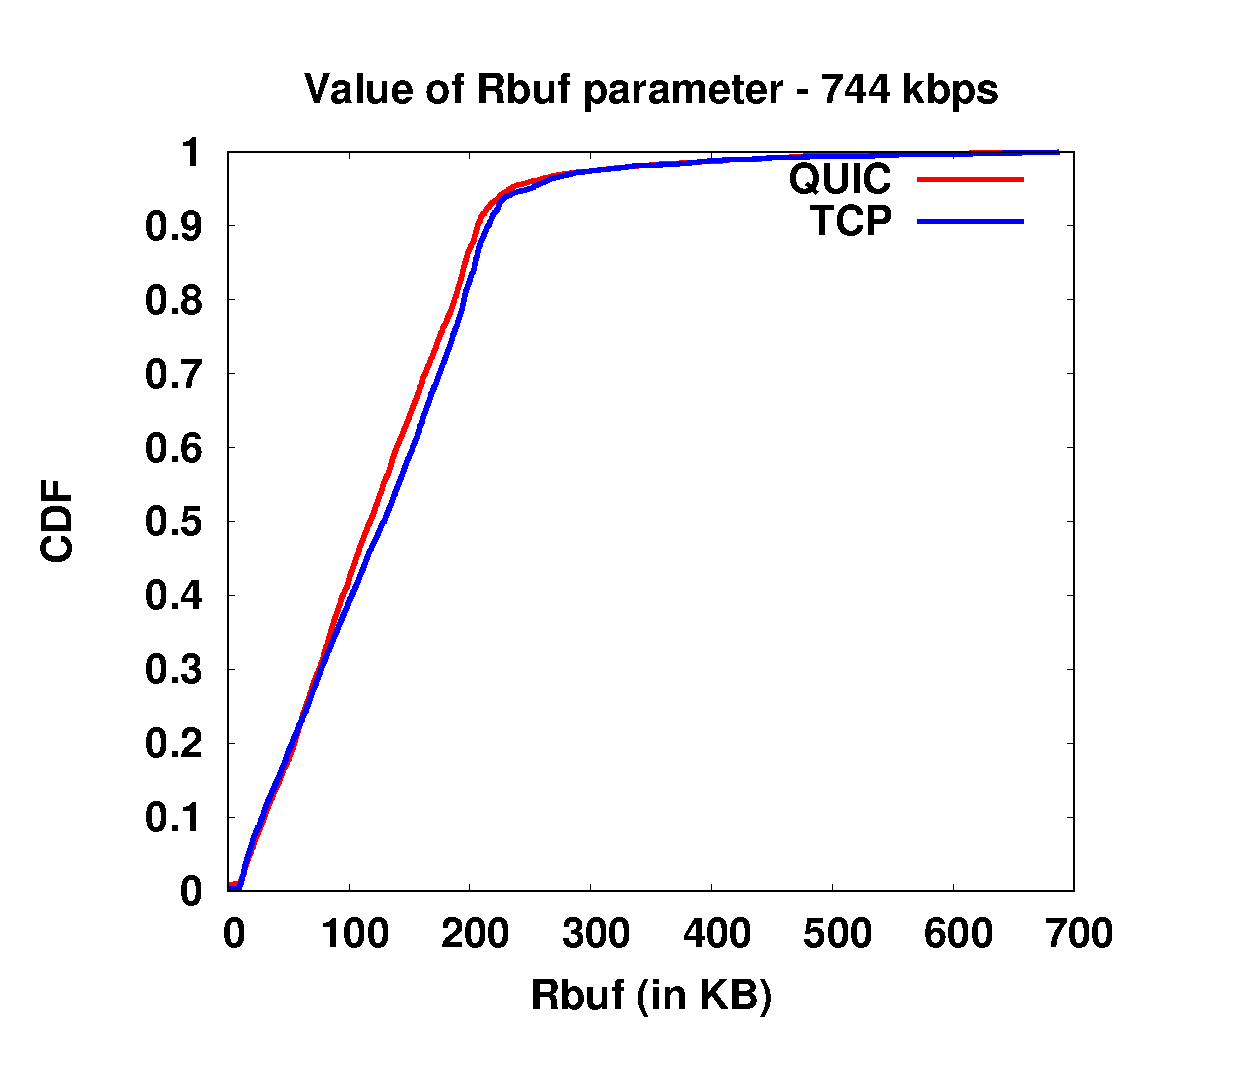
\includegraphics[width=0.9\linewidth]{img/CDF/plot_rbuf_761856}
    \caption{CDF of rbuf at 744 kbps}
    \label{fig:rbuf761856}
\end{figure}
\begin{figure}[!ht]
    \centering
    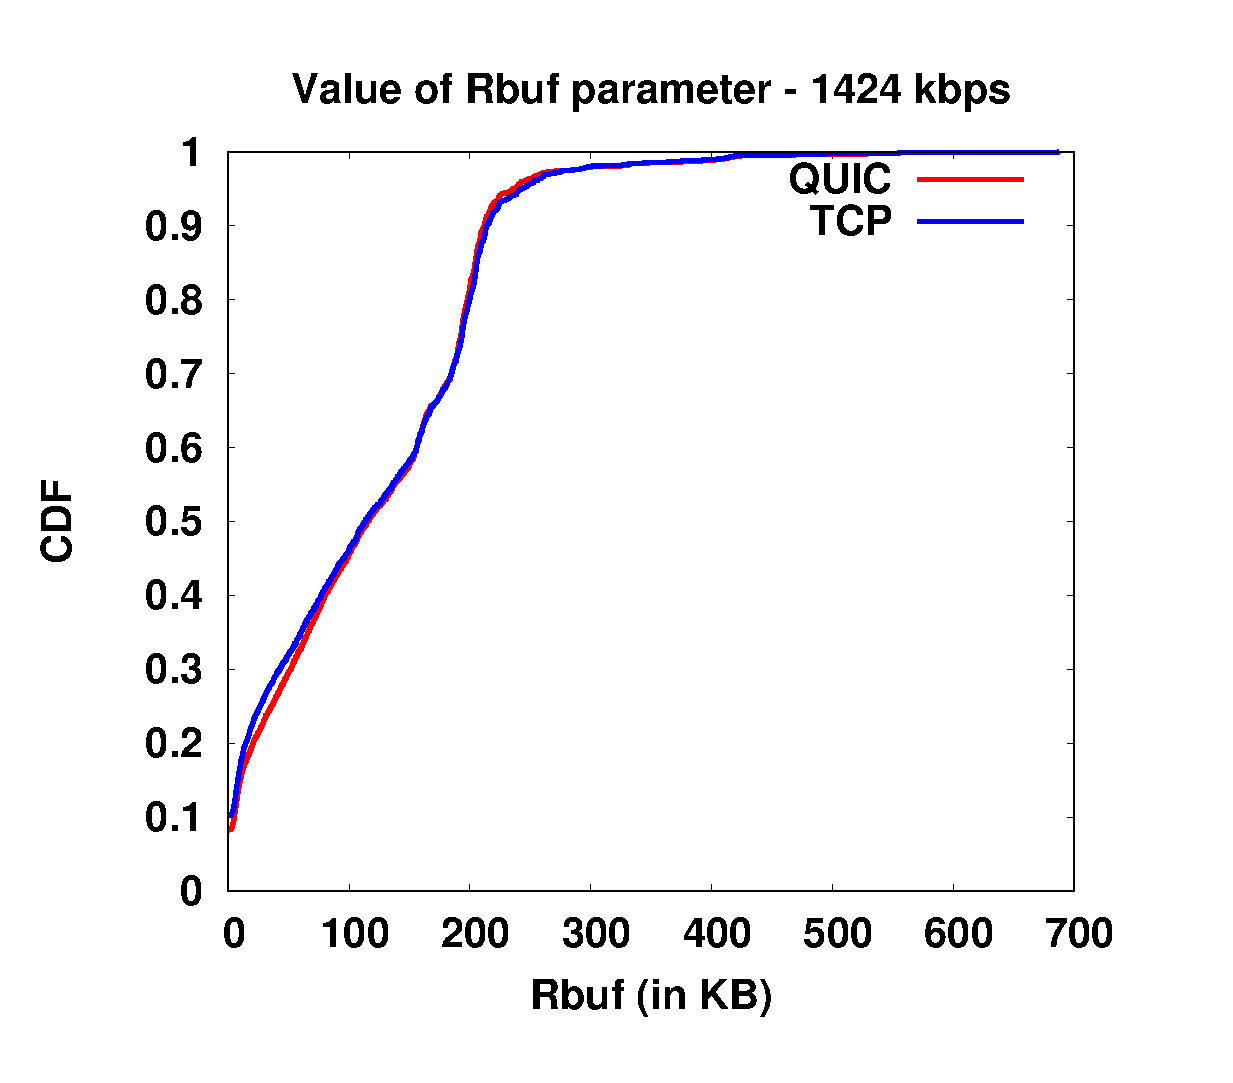
\includegraphics[width=0.9\linewidth]{img/CDF/plot_rbuf_1458176}
    \caption{CDF of rbuf at 1424 kbps}
    \label{fig:rbuf761}
\end{figure}
\end{comment}

%\subsubsection{Segment Length with respect to Various Bandwidth levels}
%As described earlier \textit{range} parameter consists of two values separated by a \\dash (-) and they define the byte range of the video for a itag value that the client requests from the server. We have taken the difference between these two values and plotted the CDF plots. At higher bandwidth levels the two protocols doesn't differ but at lower bandwidth QUIC has a greater tendency to request data in larger chunks when compared to TCP. Since QUIC is requesting in larger chunks we can estimate that it requires lesser number of requests to server to fetch data which is confirmed by the Fig. 3.8-3.10.




\begin{comment}
\begin{figure}[!ht]
    \centering
    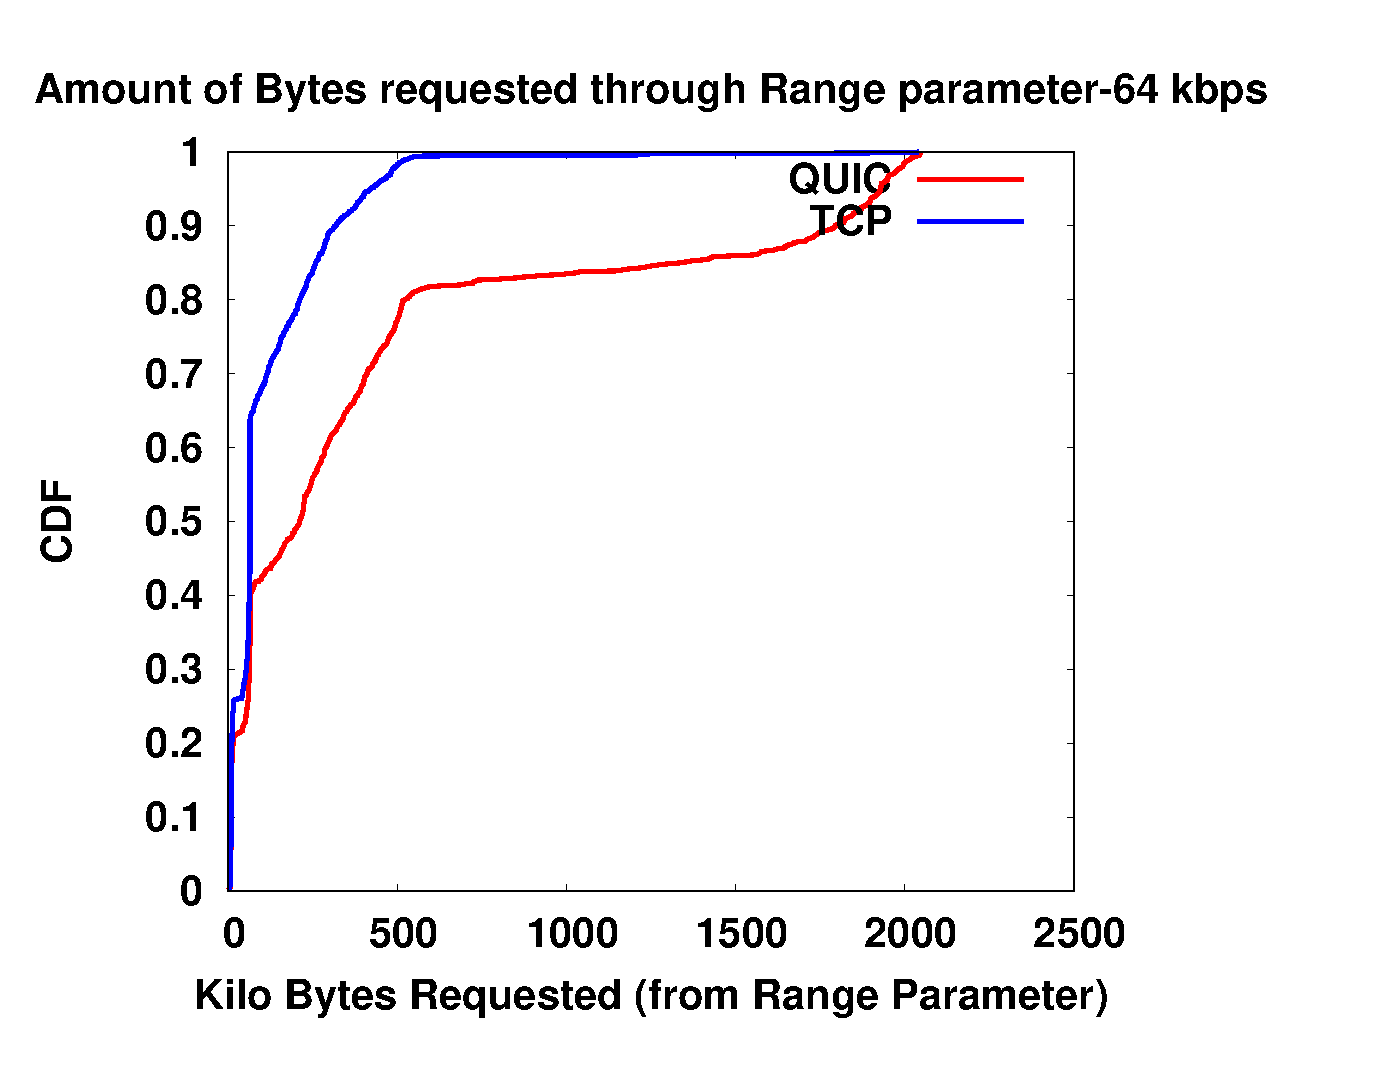
\includegraphics[width=0.9\linewidth]{img/CDF/plot_range_65536}
    \caption{CDF of range at 64 kbps}
    \label{fig:range6556}
\end{figure}
\begin{figure}[!ht]
    \centering
    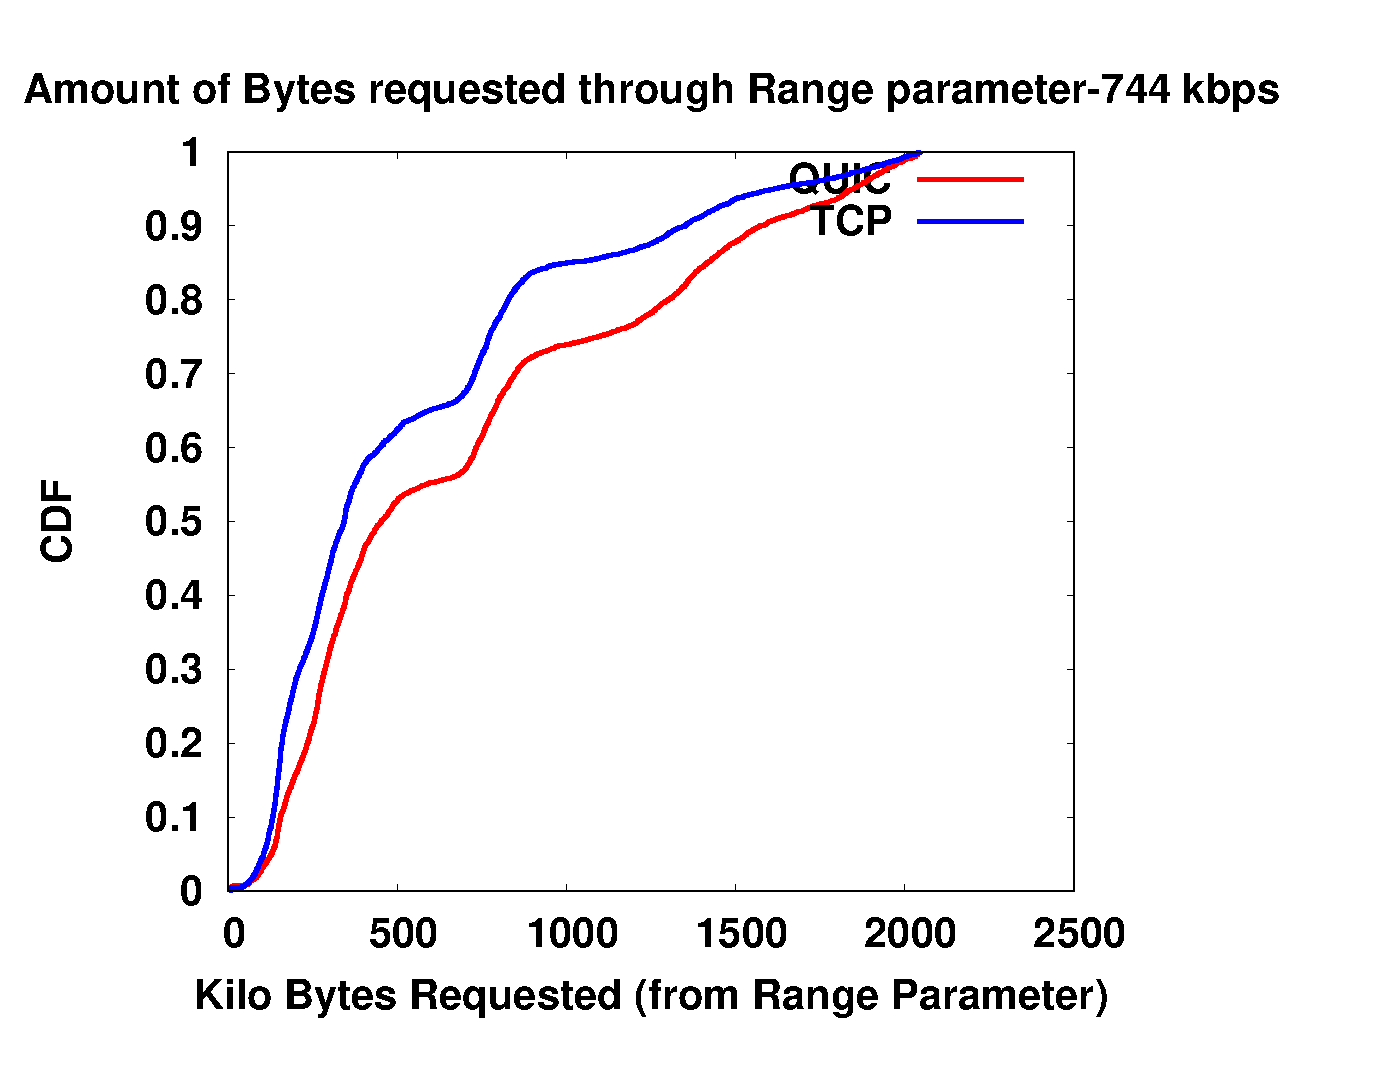
\includegraphics[width=0.9\linewidth]{img/CDF/plot_range_761856}
    \caption{CDF of range at 744 kbps}
    \label{fig:rang4761}
\end{figure}
\begin{figure}[!ht]
    \centering
    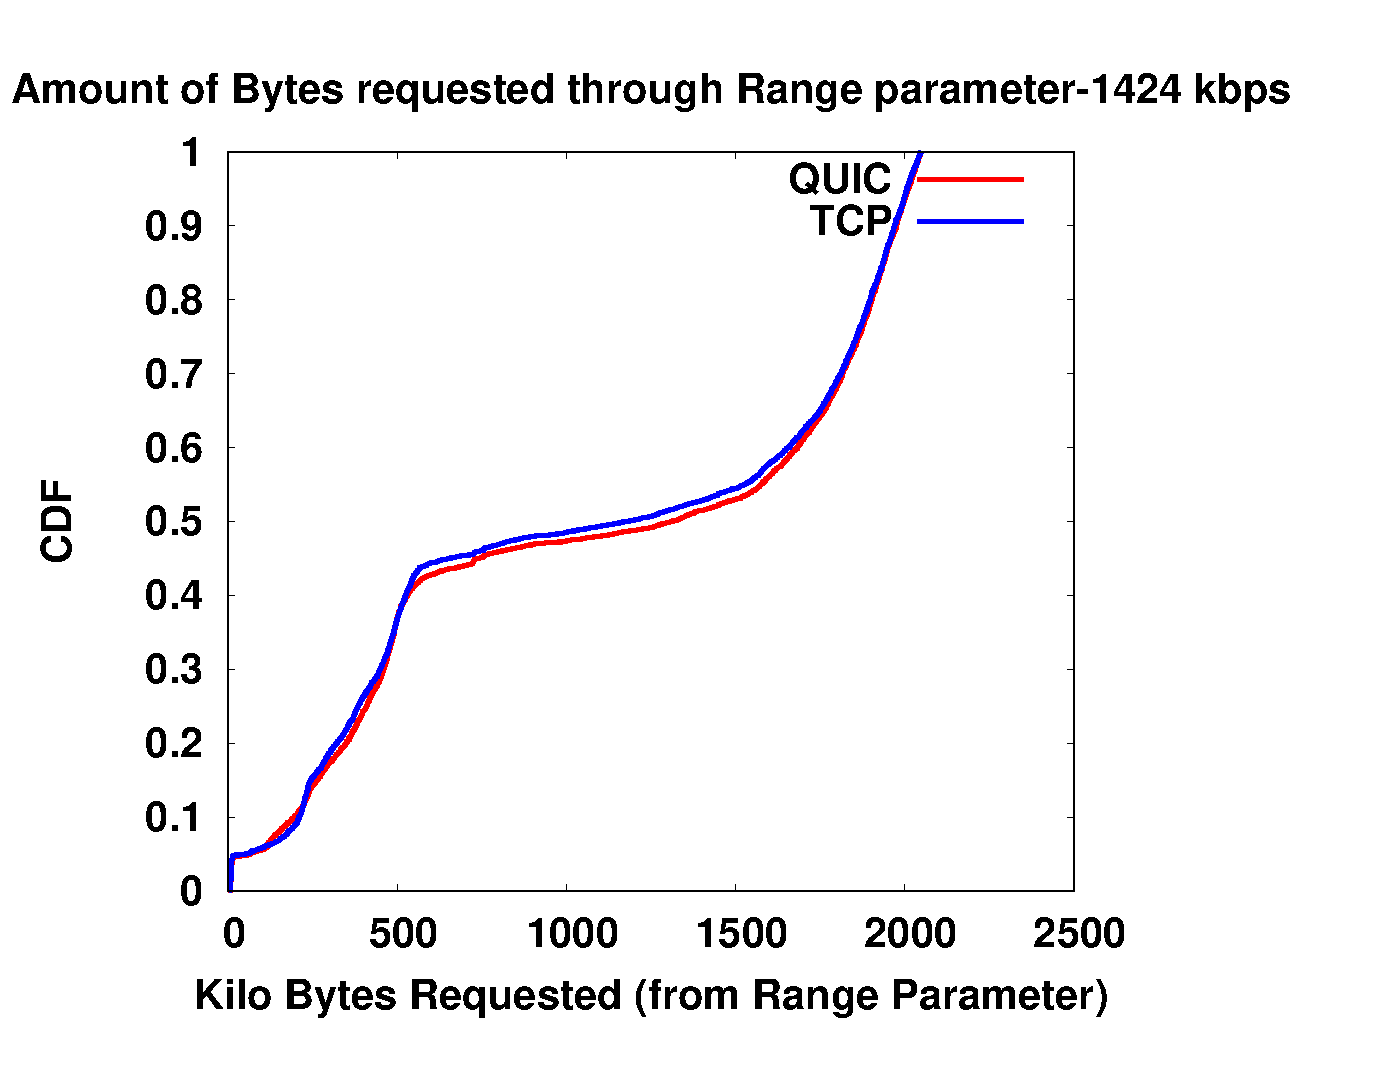
\includegraphics[width=0.9\linewidth]{img/CDF/plot_range_1458176}
    \caption{CDF of range at 1424 kbps}
    \label{fig:rang761}
\end{figure}
\end{comment}
\subsubsection{Segment Length Adaptation}

\begin{figure}[!t]
	\captionsetup[subfigure]{}
	\begin{center}
%		\subfloat[\label{fig:segment_bucket1}Bandwidth $ \leq 64 $ Kbps]{
%			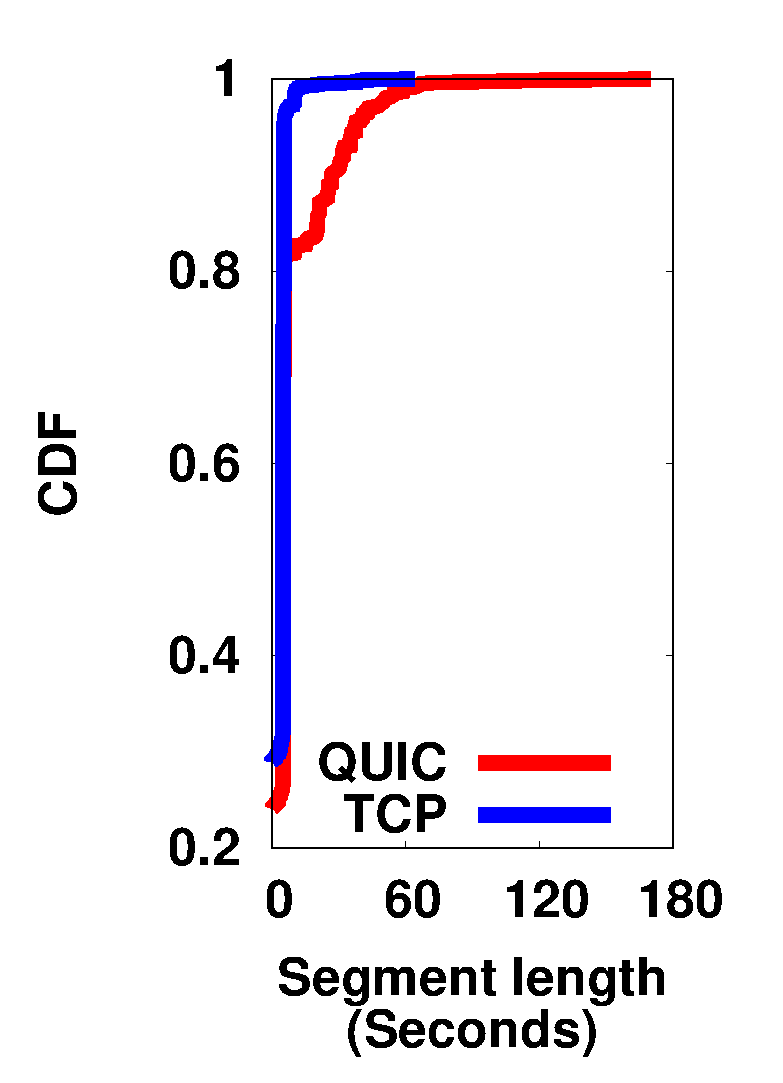
\includegraphics[width=0.32\linewidth]{img/CDF/plot_segment_bucket1}
%		}
%		\subfloat[\label{fig:segment_bucket2} $64$ Kbps $<$ Bandwidth $ \leq 1024$ Kbps]{
%			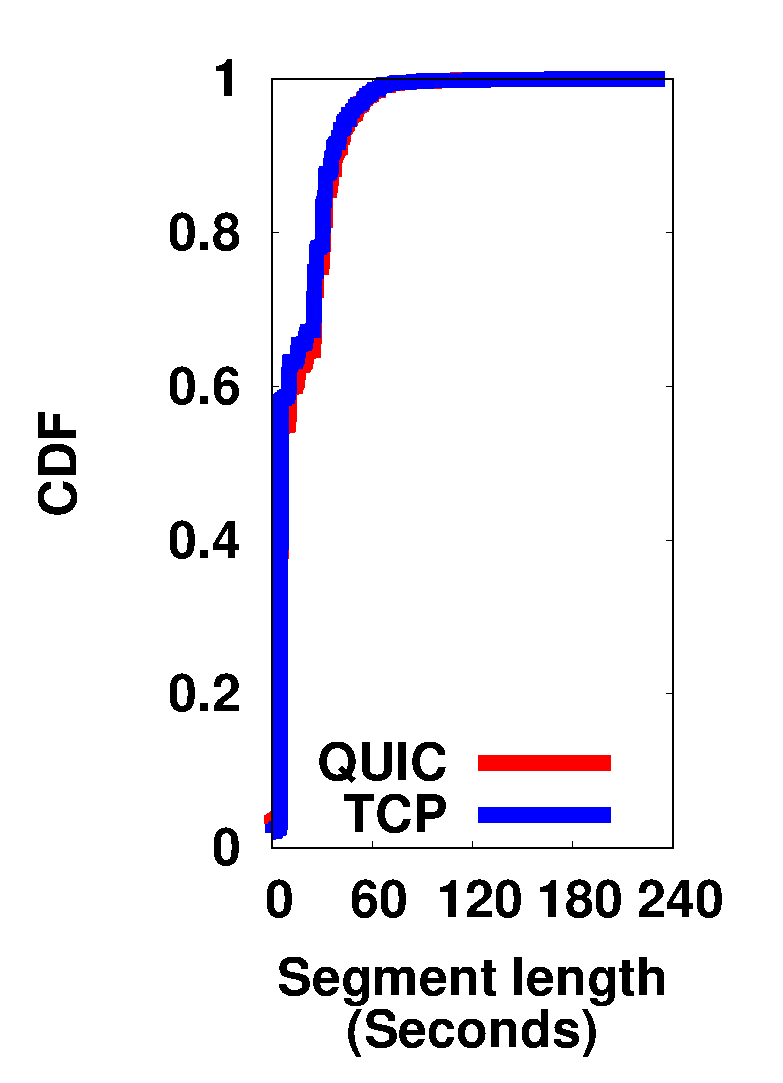
\includegraphics[width=0.32\linewidth]{img/CDF/plot_segment_bucket2}
%		}
%		\subfloat[\label{fig:segment_bucket3}Bandwidth  $> 1024$ Kbps]{
%			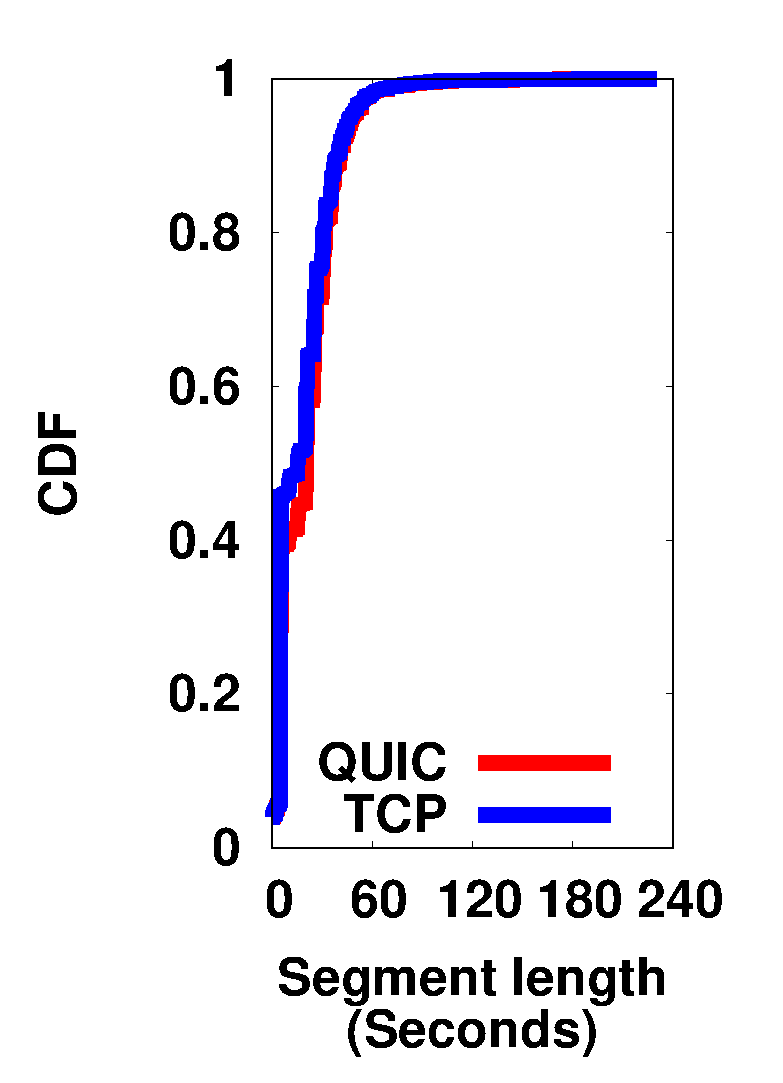
\includegraphics[width=0.32\linewidth]{img/CDF/plot_segment_bucket3}
%		}
        \includegraphics[width=\linewidth]{img/plotdata/CDF/Segment/plot_segment_bucket123}
		\caption{\label{fig:segment}Segment length with respect to various bandwidth levels: (a) $\leq 64$ Kbps, (b)  between $64$ and $1024$ Kbps, (c) $> 1024$ Kbps}
	\end{center}
\end{figure}


Apart from video quality, YouTube also adapts the segment length~\cite{mondal2017youtube} -- to download data in larger chunks when the channel condition is good. We compare the segment length adaptation behavior for \ac{QUIC} and \ac{TCP} enabled streaming in \fig\ref{fig:segment}, which shows the \ac{CDF} of segment lengths for \ac{QUIC} and \ac{TCP} enabled streaming protocols. 
%Here we observe a behavior similar to the client buffer occupancy distribution. 
Under poor channel conditions, the YouTube client tries to download data in larger chunks for \ac{QUIC} enabled streaming. This is another factor behind the increased rebuffering and comparatively high data waste with \ac{QUIC}. The fast data download capability of \ac{QUIC} does not get converted to a proper video quality adaptation feedback for the YouTube streaming mechanism, where both the quality level and the segment size of the video chunks gets adapted dynamically. 

 
%This is another way of representing the \textit{range} parameter. From the number of bytes requested through range parameter we can convert it into duration of playback seconds using the bit-rates for the \textit{itags}. The trends will be similar to the CDF plots of \textit{range} with QUIC trying to request segments with longer duration when compared to TCP at lower bandwidths but at higher bandwidths the difference is not much.

%\notesc{Merge the three plots in a single plot. (a) Bandwidth $ \leq 64 $ Kbps, (b) $64$ Kbps $<$ Bandwidth $ \leq 1024$ Kbps, (c) Bandwidth  $> 1024$ Kbps}\noteam{Done. \fig\ref{fig:segment}}

\begin{comment}
\begin{figure}[!ht]
    \centering
    \includegraphics[width=0.9\linewidth]{img/CDF/plot_segment_65536}
    \caption{CDF of Segment Length at 64 kbps}
    \label{fig:seg6556}
\end{figure}
\begin{figure}[!ht]
    \centering
    \includegraphics[width=0.9\linewidth]{img/CDF/plot_segment_761856}
    \caption{CDF of Segment Length at 744 kbps}
    \label{fig:seg7621}
\end{figure}
\begin{figure}[!ht]
    \centering
    \includegraphics[width=0.9\linewidth]{img/CDF/plot_segment_1458176}
    \caption{CDF of Segment Length at 1424 kbps}
    \label{fig:seg761}
\end{figure}
\end{comment}


\begin{comment}
%\begin{addmargin}[2.1cm]{2.1cm}
\subsubsection{CDF for \textit{itag} with respect to various \textit{rbuf} ranges(buckets) }
The two protocols does not differ much with respect to \textit{rbuf}. When the buffer is smaller in amount they fetch all the itags but when the buffer is sufficiently large both the protocols fetch data only for higher itags as it is evident in the last two plots. QUIC makes more number of requests than TCP when the client has buffered large amount of data. This can be interpreted as QUIC's estimation that since buffer has large amount of data the rate of data consumption is less when compared to data fetched so bandwidth is sufficiently good and it can make further requests. It is also evident that most of the requests to server were made when the buffer is low in data as both the protocols interpret this as data depletion at a faster rate so they try to fetch data at a faster rate which means more number of requests made.

%\end{addmargin}

\begin{figure}[!ht]
    \centering
    \includegraphics[width=0.9\linewidth]{img/CDF/plot_itag_142367}
    \caption{Number of requests and CDF of itag for rbuf $<$139 KB}
    \label{fig:itag761121}
\end{figure}

\begin{figure}[!ht]
    \centering
    \includegraphics[width=0.9\linewidth]{img/CDF/plot_itag_284734}
    \caption{Number of requests and CDF of itag for rbuf 139-278 KB}
    \label{fig:itag65526}
\end{figure}
\begin{figure}[!ht]
    \centering
    \includegraphics[width=0.9\linewidth]{img/CDF/plot_itag_427101}
    \caption{Number of requests and CDF of itag for rbuf 278-417 KB}
    \label{fig:itag7612}
\end{figure}

\begin{figure}[!ht]
    \centering
    \includegraphics[width=0.9\linewidth]{img/CDF/plot_itag_569468}
    \caption{Number of requests and CDF of itag for rbuf 417-556 KB}
    \label{fig:itag65561}
\end{figure}
\begin{figure}[!ht]
    \centering
    \includegraphics[width=0.9\linewidth]{img/CDF/plot_itag_711837}
    \caption{Number of requests and CDF of itag for rbuf 556-695 KB}
    \label{fig:itag7611}
\end{figure}

\subsubsection{CDF for \textit{range} with respect to various \textit{rbuf} ranges(buckets) }
The behaviour of both the protocols is similar when the buffer is quite low or quite high but when the buffer is in the medium range QUIC and TCP show a different pattern. When the buffer is low both the protocols take a conservative approach and request the data in smaller chunks but QUIC requests the data in a slightly larger chunks. When the buffer is above a threshold value QUIC and TCP differ in that QUIC tries to download the data in larger chunks when compared to TCP. When the buffer is sufficiently high both the protocols doesn't differ much.
\begin{figure}[!ht]
    \centering
    \includegraphics[width=0.9\linewidth]{img/CDF/plot_range_142367}
    \caption{CDF of range for rbuf $<$ 139KB}
    \label{fig:rabuf6556}
\end{figure}

\begin{figure}[!ht]
    \centering
    \includegraphics[width=0.9\linewidth]{img/CDF/plot_range_284734}
    \caption{CDF of range for rbuf 139-278KB}
    \label{fig:rabuf761856}
\end{figure}
\begin{figure}[!ht]
    \centering
    \includegraphics[width=0.9\linewidth]{img/CDF/plot_range_569468}
    \caption{CDF of range for rbuf 417-556KB}
    \label{fig:rabuf761}
\end{figure}
%\clearpage
\end{comment}



